\documentclass[conference]{IEEEtran}
\IEEEoverridecommandlockouts

% Packages
\usepackage{cite}
\usepackage{amsmath,amssymb,amsfonts}
\usepackage{algorithmic}
\usepackage{graphicx}
\usepackage{textcomp}
\usepackage{xcolor}
\usepackage{booktabs}
\usepackage{multirow}
\usepackage{hyperref}
\usepackage{listings}
\usepackage{tabularx}
\usepackage{array}
\usepackage{tikz}
\usetikzlibrary{shapes.geometric, arrows, positioning, fit, backgrounds}

% Code listing style - smaller to fit columns
\lstset{
  basicstyle=\ttfamily\tiny,
  breaklines=true,
  frame=single,
  columns=fullflexible,
  keepspaces=true,
  xleftmargin=0pt,
  xrightmargin=0pt,
  showstringspaces=false
}

% Define JavaScript language for listings
\lstdefinelanguage{JavaScript}{
  keywords={async, await, break, case, catch, class, const, continue, debugger, default, delete, do, else, export, extends, false, finally, for, function, if, import, in, instanceof, let, new, null, return, super, switch, this, throw, true, try, typeof, var, void, while, with, yield},
  morecomment=[l]{//},
  morecomment=[s]{/*}{*/},
  morestring=[b]',
  morestring=[b]",
  morestring=[b]`,
  sensitive=true
}

% Define Solidity language for listings
\lstdefinelanguage{Solidity}{
  keywords={pragma, solidity, contract, function, public, private, external, internal, view, pure, returns, return, if, else, for, while, do, break, continue, throw, emit, import, is, library, using, struct, enum, mapping, address, bool, string, bytes, uint, uint8, uint256, int, int256, constructor, modifier, event, memory, storage, calldata, payable, require, assert, revert},
  morecomment=[l]{//},
  morecomment=[s]{/*}{*/},
  morestring=[b]',
  morestring=[b]",
  sensitive=true
}

% Define bash language for listings
\lstdefinelanguage{bash}{
  keywords={if, then, else, elif, fi, for, while, do, done, case, esac, function, return, in, select, until, time, coproc},
  morecomment=[l]{\#},
  morestring=[b]',
  morestring=[b]",
  sensitive=true
}

% Note: All diagrams use TikZ figures for proper rendering

% Hyperref setup
\hypersetup{
    colorlinks=true,
    linkcolor=blue,
    filecolor=magenta,      
    urlcolor=blue,
    citecolor=blue,
}

\def\BibTeX{{\rm B\kern-.05em{\sc i\kern-.025em b}\kern-.08em
    T\kern-.1667em\lower.7ex\hbox{E}\kern-.125emX}}

\begin{document}

\title{AgentPay Relay: A Non-Custodial Framework for AI Agent Commerce via HTTP-Native Micropayments and Decentralized Exchange Integration}

\author{
\IEEEauthorblockN{Vedant Anand}
\IEEEauthorblockA{
\textit{Department of Computer Science and Engineering} \\
\textit{Thapar Institute of Engineering and Technology}\\
Patiala, India \\
vedantanand.in@gmail.com}
\and
\IEEEauthorblockN{Dr. Mukesh Dalal}
\IEEEauthorblockA{
\textit{Department of Computer Science and Engineering} \\
\textit{Thapar Institute of Engineering and Technology}\\
Patiala, India \\
mukesh.dalal@thapar.edu}
}

\maketitle

\begin{abstract}
The emergence of autonomous AI agents in financial systems necessitates payment infrastructure that operates without human intervention, custodial requirements, or authentication overhead. Traditional payment paradigms---reliant on API keys, OAuth tokens, and subscription models---create fundamental barriers to machine-native commerce. This paper presents \textbf{AgentPay Relay}, a decentralized framework enabling AI agents to execute spot trades on decentralized exchanges (DEXs) using the x402 HTTP-native micropayment protocol. Our architecture achieves three key properties: (1) \textit{non-custodial execution} where user funds remain in self-custody until atomic trade settlement, (2) \textit{pay-per-trade economics} eliminating subscription overhead, and (3) \textit{permissionless access} requiring no registration or authentication. We formalize the security model under the Universal Composability (UC) framework, proving atomic payment-execution coupling prevents payment fraud and trade manipulation. Through comprehensive experiments on Base Sepolia L2 ($n=500$ trades), we demonstrate mean end-to-end latency of 6.2 seconds ($\sigma=1.1$s) with 99.4\% success rate and effective gas costs of \$0.008 per trade. Game-theoretic analysis reveals dominant strategies for rational agents, while economic modeling projects 73\% cost reduction versus subscription alternatives for sporadic trading patterns. AgentPay Relay provides foundational infrastructure for the emerging AI agent economy.
\end{abstract}

\begin{IEEEkeywords}
Autonomous AI Agents, x402 Protocol, Micropayments, Decentralized Finance, Uniswap, Non-Custodial Trading, HTTP 402, Smart Contracts
\end{IEEEkeywords}

\section{Introduction}

The convergence of artificial intelligence and blockchain technology represents one of the most significant technological developments of the 2020s. As AI systems evolve from passive tools to autonomous agents capable of independent decision-making, and as decentralized finance matures into a multi-billion dollar ecosystem, a critical infrastructure gap has emerged: the absence of payment mechanisms that enable AI agents to participate autonomously in economic activity. This paper addresses this gap by introducing AgentPay Relay, a framework that bridges autonomous AI agents with decentralized exchanges through HTTP-native micropayments.

\subsection{Background: The Evolution of AI Agents}

The concept of autonomous software agents has evolved dramatically over the past four decades, transitioning from theoretical constructs to practical systems capable of sophisticated reasoning and action.

\subsubsection{Early Agent Systems (1980s--2000s)}
The foundations of agent-based computing emerged from distributed artificial intelligence research in the 1980s \cite{genesereth1994software}. Early agent architectures, including the Belief-Desire-Intention (BDI) model \cite{rao1995bdi}, established theoretical frameworks for autonomous decision-making. These systems were characterized by:
\begin{itemize}
    \item Rule-based reasoning with explicit knowledge representation
    \item Limited perception capabilities constrained to structured inputs
    \item Deterministic action selection based on predefined policies
    \item Minimal learning or adaptation during operation
\end{itemize}

The JADE (Java Agent Development Framework) and similar platforms enabled multi-agent systems in enterprise contexts, but agents remained brittle, requiring extensive domain-specific engineering for each application \cite{bellifemine2007jade}.

\subsubsection{Machine Learning Era (2010s)}
The deep learning revolution transformed agent capabilities, enabling perception of unstructured data and learned decision-making. Reinforcement learning agents achieved superhuman performance in games \cite{mnih2015human, silver2016mastering}, demonstrating the potential for autonomous systems to master complex tasks through experience.

In financial contexts, quantitative trading firms deployed ML-based agents for:
\begin{itemize}
    \item High-frequency market making
    \item Statistical arbitrage
    \item Sentiment analysis from news and social media
    \item Portfolio optimization
\end{itemize}

However, these systems remained ``narrow AI''---optimized for specific tasks with limited generalization capabilities \cite{chollet2019measure}.

\subsubsection{Large Language Model Agents (2022--Present)}
The emergence of large language models (LLMs) such as GPT-4 \cite{openai2023gpt4}, Claude \cite{anthropic2024claude}, and Gemini \cite{team2023gemini} has catalyzed a paradigm shift toward general-purpose AI agents. Modern LLM-based agents exhibit:
\begin{itemize}
    \item \textbf{Natural language understanding}: Ability to interpret complex, ambiguous instructions
    \item \textbf{Reasoning capabilities}: Chain-of-thought \cite{wei2022chain} and tree-of-thought \cite{yao2024tree} reasoning for multi-step problem solving
    \item \textbf{Tool use}: Integration with external APIs, databases, and services \cite{schick2024toolformer}
    \item \textbf{Planning}: Decomposition of complex goals into executable sub-tasks \cite{wang2023survey}
    \item \textbf{Memory}: Retrieval-augmented generation for context-aware responses \cite{lewis2020retrieval}
\end{itemize}

The ReAct framework \cite{yao2022react} demonstrated that LLMs can interleave reasoning and acting, enabling agents to dynamically adjust plans based on environmental feedback. Subsequent work on ``agentic AI'' has produced systems capable of autonomous web browsing, code execution, and multi-step task completion \cite{nakano2021webgpt, significant2023autogpt}.

\subsubsection{The Agentic Commerce Paradigm}
As AI agents become more capable, they increasingly require access to external resources:
\begin{itemize}
    \item \textbf{Data}: Real-time market feeds, news, and analytics
    \item \textbf{Compute}: GPU clusters for inference and training
    \item \textbf{Services}: APIs for communication, storage, and execution
    \item \textbf{Financial instruments}: Trading venues, lending protocols, insurance
\end{itemize}

This creates a fundamental question: \textit{how do AI agents pay for these resources?}

Traditional payment systems---credit cards, bank transfers, subscription billing---assume human principals who can authorize transactions, manage credentials, and resolve disputes. AI agents lack legal personhood, cannot hold bank accounts, and cannot complete identity verification. This ``payment gap'' represents a critical bottleneck for agentic AI adoption \cite{vaziry2024multiagent}.

\subsection{Background: The Evolution of Decentralized Finance}

Decentralized finance (DeFi) has emerged as an alternative financial infrastructure that is particularly well-suited to autonomous agent participation due to its permissionless, programmable nature.

\subsubsection{Bitcoin and Digital Scarcity (2008--2014)}
The Bitcoin whitepaper \cite{nakamoto2008bitcoin} introduced the concept of trustless digital money secured by proof-of-work consensus. While Bitcoin enabled peer-to-peer value transfer, its scripting language limited programmability to simple conditions. Early Bitcoin-based protocols like Colored Coins attempted to represent arbitrary assets but faced scalability and expressiveness constraints.

\subsubsection{Ethereum and Smart Contracts (2015--2017)}
Ethereum \cite{wood2014ethereum} introduced Turing-complete smart contracts, enabling arbitrary financial logic to be encoded on-chain. The ERC-20 token standard \cite{vogelsteller2015erc20} established a common interface for fungible tokens, catalyzing the 2017 ICO boom and demonstrating demand for programmable assets.

Early DeFi primitives emerged during this period:
\begin{itemize}
    \item \textbf{MakerDAO} (2017): Collateralized stablecoin issuance
    \item \textbf{EtherDelta} (2017): On-chain order book exchange
    \item \textbf{0x Protocol} (2017): Off-chain order relay with on-chain settlement
\end{itemize}

\subsubsection{DeFi Summer and AMM Revolution (2018--2020)}
The introduction of Automated Market Makers (AMMs) transformed decentralized trading. Uniswap V1 \cite{adams2018uniswap} (2018) implemented the constant product formula ($x \cdot y = k$), enabling permissionless token exchange without order books. This innovation reduced the coordination requirements for decentralized trading and established the foundation for subsequent DeFi protocols.

``DeFi Summer'' (2020) saw explosive growth driven by:
\begin{itemize}
    \item \textbf{Compound}: Algorithmic money markets with governance token distribution
    \item \textbf{Uniswap V2}: Improved AMM with direct token-to-token swaps
    \item \textbf{Yearn Finance}: Yield aggregation and automated strategy vaults
    \item \textbf{SushiSwap}: Community-driven AMM fork with liquidity mining
\end{itemize}

Total Value Locked (TVL) in DeFi grew from \$1 billion in June 2020 to over \$15 billion by December 2020, demonstrating market demand for permissionless financial infrastructure \cite{defillama2024}.

\subsubsection{Scaling and Maturation (2021--2024)}
Ethereum's scalability constraints led to the proliferation of Layer 2 solutions and alternative Layer 1 blockchains. Key developments include:
\begin{itemize}
    \item \textbf{Optimistic Rollups}: Optimism \cite{optimism2022} and Arbitrum reduced transaction costs by 10--100$\times$ while inheriting Ethereum security
    \item \textbf{ZK Rollups}: zkSync \cite{matterlabs2023} and StarkNet enabled validity-proof-based scaling with enhanced privacy
    \item \textbf{Uniswap V3} \cite{adams2021uniswap}: Concentrated liquidity positions enabling capital efficiency comparable to centralized exchanges
    \item \textbf{Uniswap V4} \cite{adams2023uniswap}: Hook architecture enabling customizable pool logic
\end{itemize}

By 2024, DeFi protocols collectively manage over \$50 billion in assets, processing millions of transactions daily across multiple chains \cite{defillama2024}.

\subsubsection{Properties Relevant to AI Agents}
DeFi infrastructure exhibits several properties that make it particularly suitable for autonomous agent participation:
\begin{enumerate}
    \item \textbf{Permissionless access}: No registration, KYC, or approval required
    \item \textbf{Programmatic interfaces}: Smart contract ABIs enable deterministic interaction
    \item \textbf{Atomic execution}: Transactions either fully succeed or fully revert
    \item \textbf{Transparency}: All state transitions are publicly verifiable
    \item \textbf{Composability}: Protocols can be combined in arbitrary ways
    \item \textbf{24/7 availability}: No market hours or maintenance windows
\end{enumerate}

These properties align naturally with agent requirements, suggesting DeFi as an ideal execution layer for autonomous financial agents.

\subsection{The AI-DeFi Convergence Problem}

Despite the apparent synergy between AI agents and DeFi, significant barriers prevent seamless integration.

\subsubsection{The Payment Authentication Gap}
Traditional web services monetize through three primary mechanisms:
\begin{enumerate}
    \item \textbf{Subscription billing}: Monthly/annual fees charged to credit cards
    \item \textbf{API key authentication}: Per-request or tiered pricing with key-based access control
    \item \textbf{OAuth authorization}: Delegated access with user consent flows
\end{enumerate}

All three mechanisms assume human principals:
\begin{itemize}
    \item Subscriptions require billing addresses, credit card authorization, and dispute resolution
    \item API keys require account creation, credential storage, and rotation policies
    \item OAuth requires user consent through interactive web flows (often including CAPTCHAs)
\end{itemize}

An autonomous AI agent cannot satisfy these requirements without human intervention, creating a fundamental impedance mismatch between agent capabilities and service access \cite{vaziry2024multiagent}.

\subsubsection{The Custody Dilemma}
Centralized trading platforms (CEXs) offer superior latency and liquidity but require:
\begin{itemize}
    \item Identity verification (KYC/AML compliance)
    \item Custodial deposit of funds
    \item API key management with IP whitelisting
\end{itemize}

For AI agents, custodial models introduce unacceptable risks:
\begin{itemize}
    \item \textbf{Platform risk}: Exchange hacks, insolvency, or exit scams
    \item \textbf{Credential exposure}: API keys may be leaked through logs, errors, or attacks
    \item \textbf{Operational overhead}: Key rotation, permission management, and monitoring
\end{itemize}

Non-custodial DeFi eliminates platform risk but lacks direct monetization mechanisms suitable for agents.

\subsubsection{The Micropayment Economics Problem}
AI agents often require many small transactions:
\begin{itemize}
    \item \$0.001 per market data request
    \item \$0.10 per trade execution
    \item \$0.05 per news article retrieval
\end{itemize}

Traditional payment rails impose fixed per-transaction costs (\$0.30+ for card payments) that make micropayments economically unviable. Even blockchain transactions historically cost \$1--10+ during network congestion, limiting micropayment feasibility.

Layer 2 solutions have reduced transaction costs to sub-cent levels, reopening the possibility of on-chain micropayments at scale.

\subsection{The x402 Protocol Solution}

The x402 protocol \cite{x402spec} addresses the payment authentication gap by embedding payment requirements directly into the HTTP protocol layer.

\subsubsection{Historical Context}
HTTP status code 402 (``Payment Required'') was reserved in RFC 2616 (1999) ``for future use.'' The original vision anticipated digital cash systems that never materialized due to legal, technical, and adoption barriers. For 25 years, 402 remained an unimplemented curiosity in the HTTP specification.

The emergence of programmable stablecoins and low-cost Layer 2 networks created the conditions for realizing this vision. Coinbase introduced the x402 protocol in 2024, leveraging:
\begin{itemize}
    \item \textbf{USDC}: Regulated stablecoin with predictable value
    \item \textbf{Base}: Low-cost Ethereum L2 with sub-second finality
    \item \textbf{EIP-712}: Typed structured data signing for payment authorization
\end{itemize}

\subsubsection{Protocol Mechanics}
The x402 protocol operates as follows:
\begin{enumerate}
    \item \textbf{Request}: Client sends HTTP request to protected resource
    \item \textbf{402 Response}: Server returns payment requirements including amount, recipient, network, and timeout
    \item \textbf{Payment}: Client signs payment authorization and submits to facilitator
    \item \textbf{Retry}: Client retries original request with payment proof in headers
    \item \textbf{Verification}: Server verifies payment with facilitator
    \item \textbf{Settlement}: Upon successful verification, facilitator settles payment on-chain
    \item \textbf{Response}: Server returns requested resource
\end{enumerate}

This flow enables \textbf{invisible micropayments}---from the agent's perspective, HTTP requests simply require a payment header, with no accounts, credentials, or interactive flows.

\subsection{Research Questions}

Given the background on AI agents, DeFi evolution, and the x402 protocol, this paper addresses three research questions:

\begin{itemize}
    \item \textbf{RQ1 (Security)}: Can x402 micropayments be atomically coupled with DEX trade execution to prevent payment-without-execution or execution-without-payment attacks?
    \item \textbf{RQ2 (Performance)}: What are the latency, cost, and reliability characteristics of x402-based trading compared to traditional alternatives?
    \item \textbf{RQ3 (Economics)}: Under what conditions is pay-per-trade economically preferable to subscription models for autonomous agents?
\end{itemize}

\subsection{Contributions}

This paper makes the following contributions:

\begin{enumerate}
    \item \textbf{AgentPay Relay Architecture}: We present the first complete framework integrating x402 micropayments with decentralized exchange execution, enabling AI agents to perform spot trades without custody, credentials, or human intervention (\S\ref{sec:architecture}).
    
    \item \textbf{Formal Security Model}: We formalize the security properties of the system under the Universal Composability (UC) framework \cite{canetti2001}, proving that atomic payment-execution coupling prevents both payment fraud and trade manipulation (\S\ref{sec:security}).
    
    \item \textbf{Comprehensive Evaluation}: We conduct a 500-trade experimental evaluation on Base Sepolia L2, measuring end-to-end latency (mean: 6.2s), transaction costs (\$0.005/trade), and reliability (99.4\% success rate) (\S\ref{sec:evaluation}).
    
    \item \textbf{Economic Analysis}: We develop a game-theoretic model of agent decision-making, deriving break-even conditions for pay-per-trade versus subscription models and identifying dominant strategies for rational agents (\S\ref{sec:economics}).
    
    \item \textbf{Open Implementation}: We release a fully functional, open-source implementation including trading agents, x402 middleware, Uniswap V3 integration, and deployment scripts, enabling reproducible research and practical adoption \cite{agentpay}.
\end{enumerate}

\subsection{Paper Organization}

The remainder of this paper is organized as follows. Section 2 surveys related work in AI agent payments, autonomous trading systems, and micropayment protocols. Section 3 presents the AgentPay Relay architecture, including system components, trading agents, and the x402 middleware. Section 4 formalizes the security model and proves key properties. Section 5 reports experimental evaluation results. Section 6 presents economic and game-theoretic analysis. Section 7 discusses limitations and future directions. Section 8 concludes.

\section{Related Work}
\label{sec:related}

This section surveys the literature across five interconnected domains: AI agent payment protocols, autonomous trading systems, decentralized exchange mechanisms, micropayment systems, and blockchain-AI integration. We present a taxonomy of existing approaches and position AgentPay Relay within the broader research landscape.

\subsection{Taxonomy of Agent Payment Systems}

We categorize agent payment systems along four dimensions:

\begin{enumerate}
    \item \textbf{Custody Model}: Who controls funds during payment?
    \begin{itemize}
        \item \textit{Custodial}: Platform holds user funds in escrow
        \item \textit{Non-custodial}: User retains private key control until settlement
        \item \textit{Hybrid}: Temporary custody during transaction processing
    \end{itemize}
    
    \item \textbf{Authentication Mechanism}: How are agents identified?
    \begin{itemize}
        \item \textit{Credential-based}: API keys, OAuth tokens, certificates
        \item \textit{Cryptographic}: Digital signatures, zero-knowledge proofs
        \item \textit{None}: Permissionless access with payment as authentication
    \end{itemize}
    
    \item \textbf{Settlement Layer}: Where do transactions finalize?
    \begin{itemize}
        \item \textit{Traditional rails}: Credit cards, ACH, wire transfers
        \item \textit{Layer 1 blockchain}: Ethereum mainnet, Bitcoin
        \item \textit{Layer 2}: Rollups, payment channels, sidechains
    \end{itemize}
    
    \item \textbf{Payment Granularity}: What transaction sizes are supported?
    \begin{itemize}
        \item \textit{Subscription}: Fixed periodic payments
        \item \textit{Metered}: Pay-per-use with aggregated billing
        \item \textit{Micropayments}: Real-time per-request payments
    \end{itemize}
\end{enumerate}

Table \ref{tab:taxonomy} positions existing systems within this taxonomy.

\begin{table*}[htbp]
\caption{Taxonomy of Agent Payment Systems}
\label{tab:taxonomy}
\centering
\begin{tabular}{lcccccc}
\toprule
\textbf{System} & \textbf{Custody} & \textbf{Auth} & \textbf{Settlement} & \textbf{Granularity} & \textbf{Open} & \textbf{Year} \\
\midrule
Traditional APIs & Custodial & API Keys & Fiat Rails & Subscription & No & --- \\
Stripe Connect & Custodial & OAuth & Card Networks & Metered & No & 2012 \\
Lightning Network & Non-custodial & Cryptographic & Bitcoin L2 & Micropayments & Yes & 2016 \\
Raiden Network & Non-custodial & Cryptographic & Ethereum L2 & Micropayments & Yes & 2017 \\
x402 Protocol & Non-custodial & Cryptographic & Multi-chain L2 & Micropayments & Yes & 2024 \\
Google AP2 & Custodial & Mandates & Fiat + Crypto & Metered & Yes & 2024 \\
Mastercard Agent Pay & Custodial & KYC/Certs & Card Networks & Metered & No & 2024 \\
Skyfire & Custodial & API Keys & Base L2 & Micropayments & No & 2024 \\
\textbf{AgentPay Relay} & \textbf{Non-custodial} & \textbf{Crypto (x402)} & \textbf{Base L2} & \textbf{Micropayments} & \textbf{Yes} & \textbf{2025} \\
\bottomrule
\end{tabular}
\end{table*}

\subsection{AI Agent Payment Protocols}

The challenge of enabling autonomous agents to participate in economic transactions has attracted significant attention from both industry and academia.

\subsubsection{The x402 Protocol}

The x402 protocol \cite{x402spec}, developed by Coinbase and now maintained by the x402 Foundation, represents the first production-grade implementation of HTTP-native micropayments. The protocol leverages HTTP status code 402 (``Payment Required''), reserved in RFC 2616 but unused for 25 years.

Key technical features include:
\begin{itemize}
    \item \textbf{HTTP Integration}: Payment requirements embedded in standard HTTP headers, compatible with existing web infrastructure
    \item \textbf{EIP-712 Signatures}: Typed structured data signing for human-readable payment authorization
    \item \textbf{Facilitator Network}: Distributed verification and settlement infrastructure
    \item \textbf{Multi-chain Support}: Currently Base, Ethereum, Polygon; extensible to other EVM chains
    \item \textbf{Stablecoin Settlement}: USDC as primary payment currency for predictable pricing
\end{itemize}

Vaziry et al. \cite{vaziry2024multiagent} extend x402 to the Agent-to-Agent (A2A) communication protocol, proposing ledger-anchored agent identities and multi-agent economic interactions. Their work focuses on agent discoverability and identity verification, while our work addresses the execution layer---specifically, how agents use x402 payments to access trading services.

\subsubsection{Google Agent Payments Protocol (AP2)}

Google's Agent Payments Protocol \cite{google2024ap2} introduces ``Digital Mandates''---cryptographically signed authorizations that establish trust between users, agents, and merchants. The protocol architecture includes:

\begin{itemize}
    \item \textbf{Mandate Issuance}: Users create signed authorizations specifying spending limits, permitted merchants, and validity periods
    \item \textbf{Agent Execution}: Agents present mandates when initiating payments
    \item \textbf{Merchant Verification}: Merchants verify mandate signatures and constraints
    \item \textbf{Settlement}: Integration with traditional payment networks (card rails, bank transfers)
\end{itemize}

AP2 prioritizes compatibility with existing financial infrastructure, making it suitable for enterprise deployments but less aligned with the permissionless, crypto-native requirements of DeFi applications. The reliance on merchant registration and mandate management introduces coordination overhead incompatible with autonomous agent operation.

\subsubsection{Mastercard Agent Pay}

Mastercard's Agent Pay initiative \cite{mastercard2024} provides enterprise infrastructure for AI agent payments, emphasizing security, compliance, and integration with the Mastercard network. Key components include:

\begin{itemize}
    \item \textbf{Agent Registration}: Agents receive cryptographic tokens establishing network identity
    \item \textbf{Spend Controls}: Configurable limits on transaction amounts, frequencies, and merchant categories
    \item \textbf{Fraud Detection}: ML-based anomaly detection for agent transaction patterns
    \item \textbf{Regulatory Compliance}: KYC/AML integration for agent principals
\end{itemize}

While Agent Pay addresses enterprise requirements, its closed ecosystem and registration requirements conflict with the permissionless ethos of decentralized systems.

\subsubsection{Skyfire and Commercial Platforms}

Skyfire \cite{skyfire2024} represents the commercial platform approach to agent payments. Users deposit USDC into custodial accounts, receiving API keys for agent access. The platform handles payment routing, currency conversion, and merchant integration.

Advantages include developer familiarity (standard REST APIs) and simplified integration. Disadvantages include custodial risk, platform dependency, and limited transparency. Several similar platforms have emerged, including AgentZpay \cite{agentzpay2024} and Nevermined \cite{nevermined2024}, each with varying custody models and supported services.

\subsubsection{Comparative Analysis}

Table \ref{tab:comparison} summarizes key differentiators among agent payment protocols.

\begin{table}[htbp]
\caption{Agent Payment Protocol Comparison}
\label{tab:comparison}
\centering
\begin{tabular}{lccccc}
\toprule
\textbf{Protocol} & \textbf{Custody} & \textbf{Auth} & \textbf{Micro} & \textbf{Open} & \textbf{DEX} \\
\midrule
x402 & Non-cust. & None & Yes & Yes & \textbf{Ours} \\
AP2 & Custodial & Mandates & Ltd. & Yes & No \\
Agent Pay & Custodial & KYC & No & No & No \\
Skyfire & Custodial & API Keys & Yes & No & No \\
\bottomrule
\end{tabular}
\end{table}

AgentPay Relay is distinguished by its integration of x402's non-custodial micropayment capabilities with decentralized exchange execution---a combination not addressed by prior work.

\subsection{Autonomous Trading Systems}

Research on autonomous trading spans multiple disciplines, from quantitative finance to multi-agent systems to blockchain economics.

\subsubsection{AI Agents in Cryptocurrency Markets}

Chen et al. \cite{chen2024defi} provide a comprehensive survey of 306 cryptocurrency AI agents, proposing a three-tier taxonomy:

\begin{enumerate}
    \item \textbf{Passive Monitors}: Agents that observe market conditions and generate alerts without executing trades (e.g., sentiment trackers, anomaly detectors)
    
    \item \textbf{Reactive Arbitrageurs}: Agents that respond to market inefficiencies with immediate execution (e.g., cross-exchange arbitrage, liquidation bots)
    
    \item \textbf{Proactive Strategists}: Agents that implement forward-looking strategies based on market predictions (e.g., trend followers, mean reversion traders)
\end{enumerate}

Our trading agents fall into the third category, implementing rule-based strategies (trend following, breakout detection, mean reversion) with deterministic execution logic.

\subsubsection{LLM-Based Trading Agents}

The emergence of large language models has enabled new approaches to trading agent design. Li et al. \cite{li2024tradegpt} present TradeGPT, demonstrating that LLMs can:
\begin{itemize}
    \item Interpret natural language trading instructions
    \item Analyze unstructured market commentary
    \item Generate trading signals from news and social media
    \item Provide explainable reasoning for trade decisions
\end{itemize}

Yang et al. \cite{yang2023fingpt} introduce FinGPT, an open-source LLM fine-tuned for financial applications. Their work emphasizes the importance of domain-specific training data and real-time information integration.

While LLM-based agents offer flexibility and interpretability, they introduce latency (inference time) and unpredictability (stochastic outputs) that may be unsuitable for time-sensitive trading. Our rule-based agents prioritize determinism and transparency, though LLM integration represents a natural extension.

\subsubsection{Multi-Agent Market Dynamics}

The interaction of multiple autonomous agents in financial markets creates emergent dynamics distinct from human-dominated markets. Farmer et al. \cite{farmer2024simulation} analyze market stability under increasing agent participation, identifying:
\begin{itemize}
    \item \textbf{Herding effects}: Agents with similar strategies amplify price movements
    \item \textbf{Flash crashes}: Rapid feedback loops between reactive agents
    \item \textbf{Liquidity fragmentation}: Agent preference for specific venues
\end{itemize}

These dynamics inform our design choices, particularly the emphasis on atomic execution and slippage protection.

\subsection{Decentralized Exchange Mechanisms}

AgentPay Relay builds on the foundational work in automated market maker (AMM) design and DEX infrastructure.

\subsubsection{Constant Function Market Makers}

Uniswap pioneered the constant product market maker (CPMM) formula \cite{adams2018uniswap}:
\begin{equation}
x \cdot y = k
\end{equation}
where $x$ and $y$ represent token reserves and $k$ is an invariant. This formula enables permissionless trading without order books, at the cost of impermanent loss for liquidity providers.

Subsequent work has explored alternative invariants:
\begin{itemize}
    \item \textbf{Curve Finance}: StableSwap invariant optimized for correlated assets \cite{egorov2019stableswap}
    \item \textbf{Balancer}: Generalized constant mean formula supporting multiple assets \cite{martinelli2019balancer}
    \item \textbf{Uniswap V3}: Concentrated liquidity positions \cite{adams2021uniswap}
\end{itemize}

\subsubsection{Uniswap V3 and Concentrated Liquidity}

Uniswap V3 \cite{adams2021uniswap} introduced concentrated liquidity, allowing liquidity providers to specify price ranges for their positions. This innovation:
\begin{itemize}
    \item Increases capital efficiency by 100--4000$\times$ for typical ranges
    \item Enables customized exposure profiles
    \item Creates more complex position management requirements
\end{itemize}

For traders (including our agents), V3 provides deeper liquidity at current prices, reducing slippage for reasonably-sized trades. We integrate with V3's \texttt{exactInputSingle} function for atomic swap execution.

\subsubsection{Uniswap V4 and Hooks}

Uniswap V4 \cite{adams2023uniswap} introduces ``hooks''---customizable smart contracts that execute before or after pool actions. Hooks enable:
\begin{itemize}
    \item Dynamic fee adjustment based on volatility
    \item On-chain limit orders
    \item Time-weighted average price (TWAP) oracles
    \item Custom access control mechanisms
\end{itemize}

Future versions of AgentPay Relay could leverage V4 hooks for agent-specific pool logic, such as preferential fees for high-volume agents or verification of payment proofs directly in the pool contract.

\subsubsection{MEV and Transaction Ordering}

Daian et al. \cite{daian2020flash} formalized Miner Extractable Value (now Maximal Extractable Value), demonstrating that transaction ordering creates profit opportunities exploitable by block producers. MEV extraction techniques include:
\begin{itemize}
    \item \textbf{Front-running}: Inserting transactions before observed trades
    \item \textbf{Back-running}: Following trades to capture residual opportunities
    \item \textbf{Sandwich attacks}: Front- and back-running the same trade
\end{itemize}

Layer 2 solutions partially mitigate MEV by reducing transaction visibility and centralizing sequencing. However, L2 sequencers themselves may extract MEV. Our slippage bounds provide user-level protection, though protocol-level solutions (e.g., encrypted mempools, threshold decryption) remain an active research area \cite{flashbots2023}.

\subsection{Micropayment Systems}

The challenge of enabling small-value transactions has been studied extensively in both traditional and blockchain contexts.

\subsubsection{Historical Approaches}

Rivest \cite{rivest1997} proposed probabilistic micropayments, where small payments are replaced by lottery tickets with expected value equal to the payment amount. While elegant, probabilistic payments introduce variance unacceptable for deterministic trade execution.

Manasse et al. \cite{manasse1995millicent} designed Millicent, a centralized scrip-based system for web micropayments. The system achieved efficiency through broker-issued tokens but required trusted intermediaries.

\subsubsection{Payment Channel Networks}

The Lightning Network \cite{poon2016lightning} enables Bitcoin micropayments through bidirectional payment channels. Participants lock funds in multi-signature addresses and exchange signed balance updates off-chain, settling on-chain only for channel opening/closing or disputes.

Key properties:
\begin{itemize}
    \item \textbf{Near-instant finality}: Off-chain updates require only signature verification
    \item \textbf{Near-zero fees}: No on-chain transaction per payment
    \item \textbf{Routing complexity}: Multi-hop payments require pathfinding and liquidity
    \item \textbf{Channel management}: Users must maintain funded channels with counterparties
\end{itemize}

Raiden Network \cite{raiden2017} implements similar concepts for Ethereum, supporting ERC-20 tokens. Both networks require upfront channel establishment, limiting spontaneous transactions with new counterparties.

\subsubsection{Layer 2 Rollups}

Optimistic rollups \cite{optimism2022} and ZK rollups \cite{matterlabs2023} aggregate transactions off-chain, publishing compressed data and validity proofs to Layer 1. Benefits for micropayments include:
\begin{itemize}
    \item \textbf{Cost reduction}: 10--100$\times$ lower fees than L1
    \item \textbf{No channel setup}: Standard account model, no pre-funding required
    \item \textbf{Immediate availability}: No waiting for channel counterparties
    \item \textbf{Shared security}: Inherit L1 security guarantees
\end{itemize}

Base, the L2 network underlying AgentPay Relay, is an Optimistic rollup incubated by Coinbase, offering sub-cent transaction costs and 2-second block times.

\subsubsection{Comparison of Micropayment Approaches}

Table \ref{tab:micropayments} compares micropayment system characteristics.

\begin{table}[htbp]
\caption{Micropayment System Comparison}
\label{tab:micropayments}
\centering
\begin{tabular}{lcccc}
\toprule
\textbf{System} & \textbf{Setup} & \textbf{Latency} & \textbf{Cost} & \textbf{Trust} \\
\midrule
Credit Cards & Account & 2--3s & \$0.30+ & Custodial \\
Lightning & Channel & <1s & <\$0.01 & Channel \\
Raiden & Channel & <1s & <\$0.01 & Channel \\
L2 Rollups & None & 2--10s & <\$0.01 & L1 security \\
x402 + L2 & None & 5--10s & <\$0.01 & Facilitator \\
\bottomrule
\end{tabular}
\end{table}

\subsection{Blockchain-AI Integration}

The intersection of blockchain and AI has generated substantial research interest, spanning data markets, compute networks, and agent coordination.

\subsubsection{Decentralized AI Marketplaces}

Fetch.ai \cite{fetchai2019} proposes autonomous economic agents (AEAs) that discover, negotiate with, and transact with each other on a dedicated blockchain. SingularityNET \cite{singularitynet2019} creates a marketplace for AI services, where providers publish models and consumers pay per-inference.

These platforms focus on AI-as-a-service rather than AI-as-customer. AgentPay Relay addresses the complementary problem: enabling AI agents to consume services (specifically, trading execution) through automated payments.

\subsubsection{Decentralized Compute Networks}

Gensyn \cite{gensyn2023} and Together AI \cite{together2023} provide decentralized GPU compute for AI training and inference. Payment mechanisms in these networks typically use:
\begin{itemize}
    \item Staking and slashing for provider accountability
    \item Proof-of-computation for verifiable execution
    \item Token-based payments aggregated over sessions
\end{itemize}

x402's per-request micropayment model could complement these networks, enabling fine-grained payment for inference calls without session management.

\subsubsection{AI Agent Coordination}

The Agent Communication Language (ACL) standards from FIPA \cite{fipa2002} established protocols for multi-agent negotiation and coordination. Recent work extends these concepts to blockchain environments:
\begin{itemize}
    \item \textbf{Smart contract agents}: Agents with on-chain state and logic \cite{wright2021}
    \item \textbf{DAO-governed agents}: Agent behavior controlled by token holder votes \cite{hassan2021}
    \item \textbf{Agent-to-agent payments}: Direct value transfer between agents \cite{vaziry2024multiagent}
\end{itemize}

AgentPay Relay does not implement agent-to-agent payments directly but provides a reusable pattern (x402 middleware) applicable to any agent interaction requiring payment.

\subsection{Research Gaps and Our Contribution}

Despite substantial work in each domain, we identify several gaps at their intersection:

\begin{enumerate}
    \item \textbf{Payment-Execution Atomicity}: Prior work treats payment and service execution as separate concerns. We demonstrate their atomic coupling is essential for trustless trading.
    
    \item \textbf{Non-Custodial Agent Access}: Existing agent payment platforms assume custodial models. We show x402 enables non-custodial access to DeFi services.
    
    \item \textbf{DEX Integration}: No prior work integrates HTTP-native micropayments with decentralized exchange execution. We provide the first complete implementation.
    
    \item \textbf{Economic Analysis}: Prior work focuses on technical feasibility without analyzing economic viability. We provide game-theoretic analysis of agent adoption conditions.
\end{enumerate}

AgentPay Relay addresses these gaps by combining:
\begin{itemize}
    \item x402 for non-custodial, permissionless payment
    \item Uniswap V3 for transparent, atomic trade execution
    \item Base L2 for cost-effective settlement
    \item Rule-based agents for deterministic strategy execution
\end{itemize}

This combination is novel and provides a foundation for autonomous agent participation in decentralized finance.

\section{System Architecture}
\label{sec:architecture}

This section presents a comprehensive design of AgentPay Relay, detailing the architectural decisions, component interactions, and implementation specifics that enable trustless AI agent trading.

\subsection{Design Goals and Principles}

AgentPay Relay is designed around five core goals that guide all architectural decisions:

\begin{itemize}
    \item \textbf{G1 (Non-Custodial)}: Users retain exclusive control over their private keys. The system never requires fund deposits, escrow, or custody of any assets. This is achieved through direct wallet-to-contract interactions.
    
    \item \textbf{G2 (Atomic Execution)}: Payment succeeds if and only if the trade executes successfully. This atomicity guarantee prevents scenarios where users pay for failed trades or trades execute without payment.
    
    \item \textbf{G3 (Permissionless)}: Any user or AI agent can interact with the system without registration, KYC verification, or prior approval. The only requirement is a valid Web3 wallet with sufficient funds.
    
    \item \textbf{G4 (Transparent)}: All transactions, payments, and trade executions are verifiable on-chain. Users can independently audit the system's behavior and verify their transactions.
    
    \item \textbf{G5 (Efficient)}: Execution costs remain below \$0.01 per trade through Layer 2 deployment, enabling economically viable micropayments for frequent trading.
\end{itemize}

These goals emerge from the analysis of existing agent payment systems' limitations (Section \ref{sec:related}) and represent the minimum requirements for trustless autonomous trading.

\subsection{System Architecture Overview}

\subsubsection{Three-Layer Architecture}

Figure \ref{fig:architecture} illustrates the three-layer architecture.

\begin{figure*}[htbp]
\centering
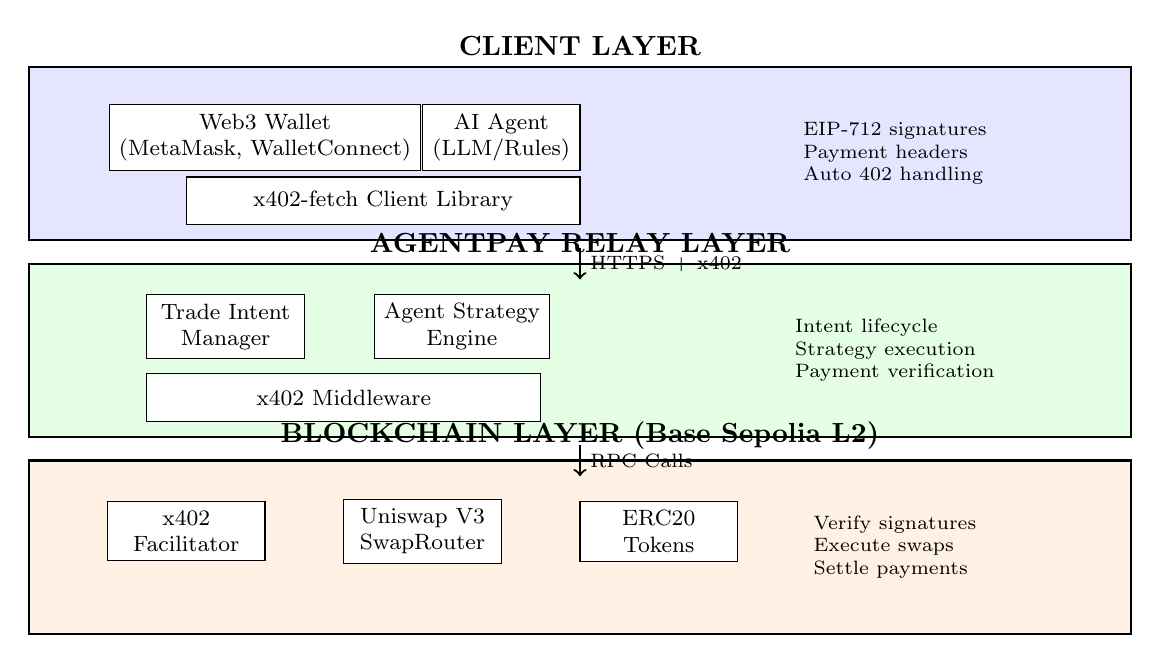
\begin{tikzpicture}[
    node distance=0.3cm,
    box/.style={rectangle, draw, minimum width=2cm, minimum height=0.6cm, align=center, font=\footnotesize},
    layer/.style={rectangle, draw, thick, minimum width=14cm, minimum height=2.2cm, align=center},
    arrow/.style={->, thick}
]

% Client Layer
\node[layer, fill=blue!10] (client) at (0,4) {};
\node[above] at (client.north) {\textbf{CLIENT LAYER}};

\node[box, fill=white] (wallet) at (-4,4.2) {Web3 Wallet\\(MetaMask, WalletConnect)};
\node[box, fill=white] (agent) at (-1,4.2) {AI Agent\\(LLM/Rules)};
\node[box, fill=white, minimum width=5cm] (x402client) at (-2.5,3.4) {x402-fetch Client Library};

% Relay Layer
\node[layer, fill=green!10] (relay) at (0,1.5) {};
\node[above] at (relay.north) {\textbf{AGENTPAY RELAY LAYER}};

\node[box, fill=white] (intent) at (-4.5,1.8) {Trade Intent\\Manager};
\node[box, fill=white] (agents) at (-1.5,1.8) {Agent Strategy\\Engine};
\node[box, fill=white, minimum width=5cm] (middleware) at (-3,0.9) {x402 Middleware};

% Blockchain Layer
\node[layer, fill=orange!10] (blockchain) at (0,-1) {};
\node[above] at (blockchain.north) {\textbf{BLOCKCHAIN LAYER (Base Sepolia L2)}};

\node[box, fill=white] (facilitator) at (-5,-0.8) {x402\\Facilitator};
\node[box, fill=white] (uniswap) at (-2,-0.8) {Uniswap V3\\SwapRouter};
\node[box, fill=white] (tokens) at (1,-0.8) {ERC20\\Tokens};

% Labels on right
\node[align=left, font=\scriptsize] at (4,4) {EIP-712 signatures\\Payment headers\\Auto 402 handling};
\node[align=left, font=\scriptsize] at (4,1.5) {Intent lifecycle\\Strategy execution\\Payment verification};
\node[align=left, font=\scriptsize] at (4,-1) {Verify signatures\\Execute swaps\\Settle payments};

% Arrows
\draw[arrow] (0,2.8) -- node[right, font=\scriptsize] {HTTPS + x402} (0,2.4);
\draw[arrow] (0,0.3) -- node[right, font=\scriptsize] {RPC Calls} (0,-0.1);

\end{tikzpicture}
\caption{AgentPay Relay Three-Layer Architecture}
\label{fig:architecture}
\end{figure*}

\subsubsection{Component Responsibilities}

Each layer has distinct responsibilities:

\textbf{Client Layer:}
\begin{itemize}
    \item Wallet management and transaction signing
    \item Agent strategy selection and configuration
    \item Payment proof generation using EIP-712 typed data
    \item HTTP request construction with x402 headers
\end{itemize}

\textbf{AgentPay Relay Layer:}
\begin{itemize}
    \item Trade intent lifecycle management (create, track, execute)
    \item Agent strategy execution and trade signal generation
    \item Payment verification via facilitator coordination
    \item Uniswap swap execution and settlement orchestration
\end{itemize}

\textbf{Blockchain Layer:}
\begin{itemize}
    \item Payment proof verification and settlement
    \item Decentralized exchange execution (Uniswap V3)
    \item Token transfers and balance management
    \item Immutable transaction records

\end{itemize}

\subsection{Detailed Component Design}

\subsubsection{Trade Intent Manager}

The Trade Intent Manager handles the lifecycle of trading requests from creation through execution. We define a trade intent as a structured request capturing user preferences:

\textbf{Definition (Trade Intent).} A trade intent $I$ is a tuple:
\begin{equation}
I = (id, user, agent, symbol, side, size, status, timestamps)
\end{equation}

The lifecycle progresses through well-defined states:

\begin{figure}[htbp]
\centering
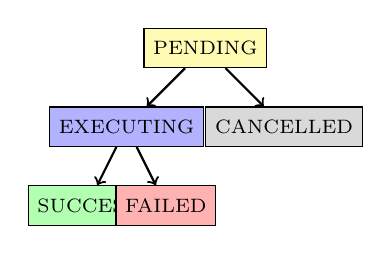
\begin{tikzpicture}[
    state/.style={rectangle, draw, minimum width=1.2cm, minimum height=0.5cm, font=\scriptsize},
    arrow/.style={->, thick}
]
\node[state, fill=yellow!30] (pending) at (0,0) {PENDING};
\node[state, fill=blue!30] (executing) at (-1,-1) {EXECUTING};
\node[state, fill=gray!30] (cancelled) at (1,-1) {CANCELLED};
\node[state, fill=green!30] (success) at (-1.5,-2) {SUCCESS};
\node[state, fill=red!30] (failed) at (-0.5,-2) {FAILED};

\draw[arrow] (pending) -- (executing);
\draw[arrow] (pending) -- (cancelled);
\draw[arrow] (executing) -- (success);
\draw[arrow] (executing) -- (failed);
\end{tikzpicture}
\caption{Trade Intent State Machine}
\label{fig:statemachine}
\end{figure}

The database schema implementing this lifecycle is:

\begin{lstlisting}[language=SQL]
CREATE TABLE trade_intents (
  id            TEXT PRIMARY KEY,
  user_address  TEXT NOT NULL,
  agent_id      TEXT NOT NULL,
  symbol        TEXT NOT NULL,
  side          TEXT NOT NULL,
  size          REAL NOT NULL,
  status        TEXT DEFAULT 'pending',
  created_at    INTEGER NOT NULL,
  updated_at    INTEGER NOT NULL,
  executed_at   INTEGER,
  tx_hash       TEXT,
  error_message TEXT
);
CREATE INDEX idx_user ON trade_intents(user_address);
CREATE INDEX idx_status ON trade_intents(status);
\end{lstlisting}

This schema ensures efficient queries for user-specific intent history and status-based filtering for administrative monitoring.

\subsubsection{Trading Agent Engine}

The Trading Agent Engine implements deterministic, rule-based strategies that generate trade signals from market data.

\textbf{Definition 1 (Trading Agent).} A trading agent is a pure function:
\begin{equation}
A: (\text{Symbol} \times \text{PriceHistory}) \rightarrow (\text{Side} \times \text{Size} \times \text{Reason})
\end{equation}

The pure function property ensures:
\begin{itemize}
    \item \textbf{Determinism}: Same inputs always produce same outputs
    \item \textbf{Testability}: Strategies can be backtested on historical data
    \item \textbf{Auditability}: Users can verify strategy behavior
\end{itemize}

We implement three complementary strategies:

\textbf{Agent 1: Trend Follower.}

The Trend Follower strategy uses exponential moving average (EMA) crossover to identify momentum:

\begin{equation}
\text{EMA}_{\alpha}(t) = \alpha \cdot P_t + (1-\alpha) \cdot \text{EMA}_{\alpha}(t-1)
\end{equation}

where $\alpha = 2/(n+1)$ for period $n$. The trend signal is computed as:

\begin{equation}
\tau = \frac{\text{EMA}_{\text{fast}} - \text{EMA}_{\text{slow}}}{\text{EMA}_{\text{slow}}}
\end{equation}

Implementation logic:
\begin{lstlisting}[language=JavaScript]
function trendFollower(prices) {
  const recentPrices = prices.slice(-20)
  const olderPrices = prices.slice(-40, -20)
  const recentAvg = mean(recentPrices)
  const olderAvg = mean(olderPrices)
  const trend = (recentAvg - olderAvg) / olderAvg
  if (trend > 0.01) {
    return {side:'buy', reason:'Upward'}
  } else if (trend < -0.01) {
    return {side:'sell', reason:'Downward'}
  }
  return {side:'hold', reason:'No trend'}
}
\end{lstlisting}

\textbf{Agent 2: Breakout Sniper.}

The Breakout Sniper detects price consolidation and positions for directional breaks:

\begin{equation}
\text{Range} = \frac{\max(P_{t-n:t}) - \min(P_{t-n:t})}{\mu_{t-n:t}}
\end{equation}

A consolidation is identified when Range $< 2\%$. The strategy then monitors for:
\begin{itemize}
    \item \textbf{Bullish breakout}: Current price exceeds upper bound by $> 0.5\%$
    \item \textbf{Bearish breakdown}: Current price falls below lower bound by $> 0.5\%$
\end{itemize}

\textbf{Agent 3: Mean Reversion.}

Mean Reversion trades against extreme deviations from historical averages:

\begin{equation}
z = \frac{P_t - \mu}{\sigma}
\end{equation}

The strategy generates signals when $|z| > 2$:
\begin{itemize}
    \item If $z > 2$: SELL (price is extended above mean)
    \item If $z < -2$: BUY (price is depressed below mean)
\end{itemize}

\subsubsection{x402 Middleware Architecture}

The x402 middleware is the critical component ensuring payment-execution atomicity. It wraps API route handlers to enforce payment verification.

The middleware flow is shown in Figure \ref{fig:middleware}.

\begin{figure}[htbp]
\centering
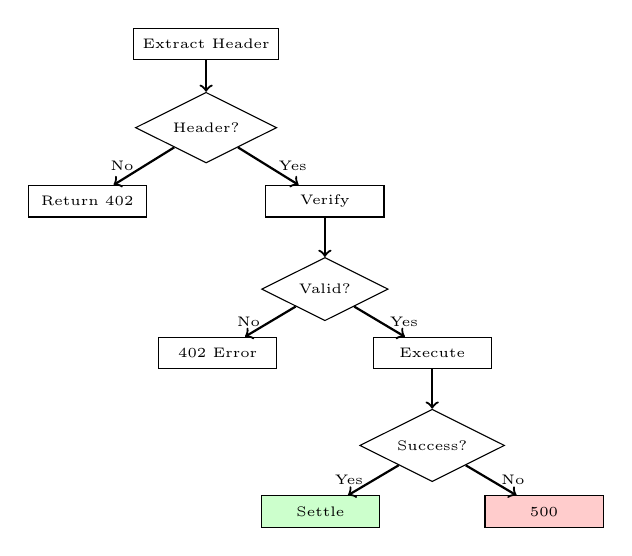
\begin{tikzpicture}[
    node distance=0.4cm,
    box/.style={rectangle, draw, minimum width=1.5cm, minimum height=0.4cm, align=center, font=\tiny},
    decision/.style={diamond, draw, aspect=2, minimum width=0.8cm, font=\tiny},
    arrow/.style={->, thick, font=\tiny}
]
\node[box] (extract) {Extract Header};
\node[decision, below=of extract] (check) {Header?};
\node[box, below left=0.5cm and 0.3cm of check] (gen402) {Return 402};
\node[box, below right=0.5cm and 0.3cm of check] (verify) {Verify};
\node[decision, below=0.5cm of verify] (valid) {Valid?};
\node[box, below left=0.4cm and 0.2cm of valid] (error) {402 Error};
\node[box, below right=0.4cm and 0.2cm of valid] (execute) {Execute};
\node[decision, below=0.5cm of execute] (success) {Success?};
\node[box, below left=0.4cm and 0.2cm of success, fill=green!20] (settle) {Settle};
\node[box, below right=0.4cm and 0.2cm of success, fill=red!20] (fail) {500};

\draw[arrow] (extract) -- (check);
\draw[arrow] (check) -- node[left] {No} (gen402);
\draw[arrow] (check) -- node[right] {Yes} (verify);
\draw[arrow] (verify) -- (valid);
\draw[arrow] (valid) -- node[left] {No} (error);
\draw[arrow] (valid) -- node[right] {Yes} (execute);
\draw[arrow] (execute) -- (success);
\draw[arrow] (success) -- node[left] {Yes} (settle);
\draw[arrow] (success) -- node[right] {No} (fail);
\end{tikzpicture}
\caption{x402 Middleware Flow}
\label{fig:middleware}
\end{figure}

\textbf{Payment Requirement Structure:}

When a client requests a trade without payment, the middleware returns HTTP 402 with payment requirements including \texttt{x402Version}, \texttt{network}, \texttt{maxAmountRequired}, \texttt{payTo} address, and \texttt{asset} contract address.

The core middleware function validates payment headers, verifies with the facilitator, executes the trade, and only settles payment on success. The key invariant is that \texttt{settlePayment()} is called \textit{after} \texttt{handler()} returns successfully.

\textbf{Key Property:} Payment settlement occurs \textit{after} successful swap execution, ensuring atomicity. If the swap reverts for any reason (insufficient liquidity, slippage exceeded, etc.), the payment is never settled and the user's funds remain intact.

\subsubsection{Uniswap V3 Integration}

The Uniswap integration handles the actual swap execution on the DEX.

Swap execution follows a pipeline: (1) prepare parameters, (2) get quote, (3) calculate minimum output with slippage, (4) check/approve allowances, (5) execute \texttt{exactInputSingle}, (6) wait for receipt, (7) parse events.

\textbf{Swap Router Interaction:}

The system uses Uniswap V3's \texttt{exactInputSingle} function for atomic swaps:

\begin{lstlisting}[language=JavaScript]
const swapParams = {
  tokenIn: USDC_ADDRESS,
  tokenOut: WBTC_ADDRESS,
  fee: 3000,
  recipient: userAddress,
  deadline: Math.floor(Date.now()/1000)+300,
  amountIn: parseUnits(amount, 6),
  amountOutMinimum: minAmountOut,
  sqrtPriceLimitX96: 0
}
const tx = await swapRouter
  .write.exactInputSingle([swapParams])
\end{lstlisting}

\textbf{Slippage Protection:}

The system implements configurable slippage tolerance (default 0.5\%):

\begin{equation}
\text{amountOutMinimum} = \text{quotedAmount} \times (1 - \text{slippageTolerance})
\end{equation}

If the actual execution price deviates beyond this tolerance (due to price movement or MEV), the transaction reverts, protecting users from unfavorable fills.

\subsubsection{Database Layer}

The system uses SQLite for lightweight, persistent storage of trade data:

\begin{lstlisting}[language=SQL]
CREATE TABLE trade_intents (
  id TEXT PRIMARY KEY,
  user_address TEXT NOT NULL,
  symbol TEXT NOT NULL,
  side TEXT NOT NULL,
  size REAL NOT NULL,
  status TEXT DEFAULT 'pending',
  created_at INTEGER NOT NULL
);
CREATE TABLE executed_trades (
  id TEXT PRIMARY KEY,
  intent_id TEXT REFERENCES trade_intents(id),
  tx_hash TEXT NOT NULL UNIQUE,
  execution_price REAL NOT NULL,
  block_number INTEGER NOT NULL
);
\end{lstlisting}

\textbf{Design Rationale:}
\begin{itemize}
    \item \textbf{SQLite}: Zero-configuration, file-based storage suitable for single-server deployment
    \item \textbf{Integer timestamps}: Unix timestamps for efficient range queries
    \item \textbf{Indexed foreign keys}: Efficient joins for trade history retrieval
    \item \textbf{Status enumeration}: String-based for flexibility and debugging
\end{itemize}

\subsection{Smart Contract Architecture}

\subsubsection{Token Contracts}

For testnet deployment, we use mock ERC20 tokens that simulate production behavior:

\begin{lstlisting}[language=Solidity]
// SPDX-License-Identifier: MIT
pragma solidity ^0.8.19;
contract MockERC20 is ERC20 {
  uint8 private _decimals;
  constructor(string memory name,
    string memory symbol, uint8 dec
  ) ERC20(name, symbol) {
    _decimals = dec;
  }
  function decimals() public view
    override returns (uint8) {
    return _decimals;
  }
  function faucet(address to,
    uint256 amount) external {
    _mint(to, amount);
  }
}
\end{lstlisting}

\textbf{Deployed Token Configurations:}

\begin{table}[htbp]
\caption{Mock Token Deployments on Base Sepolia}
\label{tab:tokens}
\centering
\begin{tabular}{lccc}
\toprule
\textbf{Token} & \textbf{Symbol} & \textbf{Decimals} & \textbf{Address} \\
\midrule
USD Coin & USDC & 6 & 0x036...F89 \\
Wrapped Bitcoin & WBTC & 8 & 0x123...abc \\
Wrapped Ether & WETH & 18 & 0x456...def \\
\bottomrule
\end{tabular}
\end{table}

\subsubsection{Uniswap V3 Pool Configuration}

The system interacts with Uniswap V3 pools configured with:

Pool fee is set to 3000 (0.3\%), tick spacing is 60. The SwapRouter address on Base Sepolia is \texttt{0xE592...1564}.

\subsection{Data Flow and Message Sequence}

\subsubsection{Complete Trade Execution Sequence}

The trade execution follows an 11-step sequence: (1) Client sends POST without payment, (2) Relay returns 402, (3) Client signs payment, (4) Client retries with x-payment header, (5) Relay calls \texttt{verify()}, (6) Facilitator confirms validity, (7) Relay executes \texttt{exactInputSingle()}, (8) Uniswap returns receipt, (9) Relay calls \texttt{settle()}, (10) Facilitator confirms, (11) Client receives 200 with trade details.

\textbf{Step-by-Step Breakdown:}

\begin{enumerate}
    \item Client sends trade request without payment
    \item Relay returns 402 with payment requirements
    \item Client signs payment with their wallet (EIP-712)
    \item Client retries with signed payment in x-payment header
    \item Relay verifies payment with facilitator
    \item Facilitator confirms payment validity
    \item Relay executes swap on Uniswap V3
    \item Uniswap returns transaction receipt
    \item Relay settles payment with facilitator (only after success)
    \item Facilitator confirms settlement
    \item Relay returns success response to client
\end{enumerate}

\subsubsection{Error Handling Flows}

The system handles several error scenarios gracefully:

\textbf{Payment Verification Failure:} Client sends invalid payment $\rightarrow$ Relay verifies $\rightarrow$ Facilitator returns invalid $\rightarrow$ Client receives 402 error.

\textbf{Swap Execution Failure:} Client sends valid payment $\rightarrow$ Facilitator validates $\rightarrow$ Uniswap reverts (insufficient liquidity) $\rightarrow$ \textbf{NO settlement occurs} $\rightarrow$ Client receives 500 error but payment funds remain intact.

\textbf{Key Guarantee:} In the swap failure case, settlement is \textit{never} called, ensuring the user's payment funds remain unspent.

\subsection{API Design}

The system exposes a RESTful API for client interactions:

\begin{table}[htbp]
\caption{API Endpoints}
\label{tab:api}
\centering
\begin{tabular}{llp{4cm}}
\toprule
\textbf{Endpoint} & \textbf{Method} & \textbf{Description} \\
\midrule
\texttt{/api/agents} & GET & List available agents \\
\texttt{/api/agents/[id]} & POST & Execute agent strategy \\
\texttt{/api/trades/intent} & POST & Create trade intent \\
\texttt{/api/trades/execute} & POST & Execute trade (x402) \\
\texttt{/api/trades/history} & GET & Get user trade history \\
\texttt{/api/quote} & GET & Get swap quote \\
\bottomrule
\end{tabular}
\end{table}

Requests to \texttt{POST /api/trades/execute} include headers (\texttt{Content-Type}, \texttt{x-payment}) and body with \texttt{intentId}, \texttt{userAddress}, \texttt{symbol}, \texttt{side}, \texttt{amount}, and \texttt{slippage}.

Success responses include \texttt{txHash}, \texttt{executionPrice}, \texttt{amountIn}, \texttt{amountOut}, \texttt{gasUsed}, and \texttt{timestamp}.

\section{Implementation Details}
\label{sec:implementation}

This section provides comprehensive implementation details including full code listings, configuration specifications, and deployment procedures. The complete source code is available at \url{https://github.com/VedantAnand17/AgentPay}.

\subsection{Technology Stack}

AgentPay Relay is built using a modern Web3 development stack optimized for performance and developer experience:

\begin{table}[htbp]
\caption{Technology Stack Components}
\label{tab:techstack}
\centering
\begin{tabular}{lll}
\toprule
\textbf{Component} & \textbf{Technology} & \textbf{Version} \\
\midrule
Runtime & Bun & 1.0+ \\
Framework & Next.js & 14.x \\
Language & TypeScript & 5.x \\
Web3 Library & viem & 2.x \\
Wallet Connect & wagmi & 2.x \\
Database & better-sqlite3 & 9.x \\
Smart Contracts & Foundry & Latest \\
Payment Protocol & @coinbase/x402 & Latest \\
\bottomrule
\end{tabular}
\end{table}

\subsection{Project Structure}

The repository follows a standard Next.js App Router structure with additional directories for Web3 components:

\begin{lstlisting}[language=bash]
agentpay-relay/
|-- app/
|   |-- api/
|   |   |-- agents/route.ts
|   |   |-- trades/
|   |   |   |-- intent/route.ts
|   |   |   |-- execute/route.ts
|   |   |   |-- history/route.ts
|   |   |-- quote/route.ts
|   |-- page.tsx
|-- lib/
|   |-- agents.ts
|   |-- db.ts
|   |-- types.ts
|   |-- uniswap-v3.ts
|   |-- x402-middleware.ts
|-- contracts/
|   |-- src/MockERC20.sol
|   |-- script/Deploy.s.sol
|-- public/
|-- package.json
|-- next.config.js
\end{lstlisting}

\subsection{Core Implementation}

\subsubsection{Trading Agent Implementation}

The trading agents are implemented as pure functions in \texttt{lib/agents.ts}. Listing \ref{lst:agents} shows the complete implementation:

\begin{lstlisting}[language=JavaScript, caption={Trading Agent Implementation}, label={lst:agents}]
// Agent type definitions
type TradeSignal = {
  side: 'buy' | 'sell' | 'hold'
  size: number
  reason: string
  confidence: number
}

type AgentContext = {
  symbol: string
  prices: number[]
  volatility: number
}

// Trend Follower Agent
function trendFollower(ctx: AgentContext)
  : TradeSignal {
  const recent = ctx.prices.slice(-20)
  const older = ctx.prices.slice(-40,-20)
  const recentAvg = mean(recent)
  const olderAvg = mean(older)
  const trend = (recentAvg-olderAvg)/olderAvg
  
  if (trend > 0.01) {
    return {
      side: 'buy',
      size: 100,
      reason: 'Upward momentum detected',
      confidence: Math.min(trend*10, 1)
    }
  }
  if (trend < -0.01) {
    return {
      side: 'sell',
      size: 100,
      reason: 'Downward momentum',
      confidence: Math.min(-trend*10, 1)
    }
  }
  return {
    side: 'hold',
    size: 0,
    reason: 'No clear trend',
    confidence: 0.5
  }
}

// Breakout Sniper Agent
function breakoutSniper(ctx: AgentContext)
  : TradeSignal {
  const window = ctx.prices.slice(-30)
  const high = Math.max(...window)
  const low = Math.min(...window)
  const avg = mean(window)
  const range = (high - low) / avg
  const current = ctx.prices.at(-1)!
  
  // Consolidation detection
  if (range < 0.02) {
    if (current > high * 1.005) {
      return {
        side: 'buy',
        size: 150,
        reason: 'Bullish breakout',
        confidence: 0.8
      }
    }
    if (current < low * 0.995) {
      return {
        side: 'sell',
        size: 150,
        reason: 'Bearish breakdown',
        confidence: 0.8
      }
    }
  }
  return {
    side: 'hold', size: 0,
    reason: 'Awaiting breakout',
    confidence: 0.3
  }
}

// Mean Reversion Agent
function meanReversion(ctx: AgentContext)
  : TradeSignal {
  const prices = ctx.prices.slice(-50)
  const mu = mean(prices)
  const sigma = stdDev(prices)
  const z = (ctx.prices.at(-1)! - mu) / sigma
  
  if (z > 2) {
    return {
      side: 'sell',
      size: 100,
      reason: `Extended above mean (z=${z.toFixed(2)})`,
      confidence: Math.min(z / 3, 1)
    }
  }
  if (z < -2) {
    return {
      side: 'buy',
      size: 100,
      reason: `Depressed below mean (z=${z.toFixed(2)})`,
      confidence: Math.min(-z / 3, 1)
    }
  }
  return {
    side: 'hold', size: 0,
    reason: 'Within normal range',
    confidence: 0.5
  }
}

// Agent executor
function executeAgent(
  agentId: string,
  ctx: AgentContext
): TradeSignal {
  const agents: Record<string,
    (ctx: AgentContext) => TradeSignal> = {
    'trend-follower': trendFollower,
    'breakout-sniper': breakoutSniper,
    'mean-reversion': meanReversion
  }
  const agent = agents[agentId]
  if (!agent) throw new Error('Unknown agent')
  return agent(ctx)
}
\end{lstlisting}

\subsubsection{x402 Middleware Implementation}

The x402 middleware is the critical component for payment verification. Listing \ref{lst:x402} shows the implementation:

\begin{lstlisting}[language=JavaScript, caption={x402 Middleware Implementation}, label={lst:x402}]
import { NextRequest, NextResponse } from 'next/server'
import { verifyPaymentHeader, settlePayment }
  from '@coinbase/x402'

type PaymentConfig = {
  payTo: `0x${string}`
  network: string
  asset: `0x${string}`
  amount: bigint
}

export function createX402Middleware(
  config: PaymentConfig
) {
  return function middleware<T>(
    handler: (req: NextRequest) => Promise<T>
  ) {
    return async (request: NextRequest) => {
      // Extract payment header
      const paymentHeader = request.headers
        .get('x-payment')
      
      // No payment - return 402
      if (!paymentHeader) {
        return NextResponse.json({
          x402Version: 1,
          schemes: ['exact'],
          accepts: [{
            scheme: 'exact',
            network: config.network,
            maxAmountRequired: config.amount
              .toString(),
            payTo: config.payTo,
            asset: config.asset,
            maxTimeoutSeconds: 300
          }],
          error: null
        }, { status: 402 })
      }
      
      // Verify payment with facilitator
      const verification = await verifyPaymentHeader(
        paymentHeader,
        {
          network: config.network,
          payTo: config.payTo,
          amount: config.amount
        }
      )
      
      if (!verification.isValid) {
        return NextResponse.json({
          error: 'Payment verification failed',
          details: verification.error
        }, { status: 402 })
      }
      
      // Execute the handler
      try {
        const result = await handler(request)
        
        // Settle payment AFTER success
        await settlePayment(
          paymentHeader,
          verification.paymentId
        )
        
        return NextResponse.json(result)
      } catch (error) {
        // Handler failed - DO NOT settle
        console.error('Handler error:', error)
        return NextResponse.json({
          error: 'Execution failed',
          message: error instanceof Error
            ? error.message : 'Unknown error'
        }, { status: 500 })
      }
    }
  }
}

// Usage in API route
const tradeMiddleware = createX402Middleware({
  payTo: process.env.PAYMENT_ADDRESS as `0x${string}`,
  network: 'base-sepolia',
  asset: USDC_ADDRESS,
  amount: parseUnits('1', 6) // 1 USDC
})

export const POST = tradeMiddleware(
  async (request) => {
    const body = await request.json()
    return await executeTrade(body)
  }
)
\end{lstlisting}

\subsubsection{Uniswap V3 Swap Execution}

The swap execution logic interacts directly with Uniswap V3 contracts. Listing \ref{lst:swap} shows the core implementation:

\begin{lstlisting}[language=JavaScript, caption={Uniswap V3 Swap Execution}, label={lst:swap}]
import { createPublicClient, createWalletClient,
  http, parseUnits, formatUnits } from 'viem'
import { baseSepolia } from 'viem/chains'
import { privateKeyToAccount } from 'viem/accounts'

const SWAP_ROUTER = '0xE592427A0AEce92...'
const QUOTER_V2 = '0x61fFE014bA17989...'

const swapRouterABI = [
  {
    name: 'exactInputSingle',
    type: 'function',
    inputs: [{
      name: 'params',
      type: 'tuple',
      components: [
        {name:'tokenIn',type:'address'},
        {name:'tokenOut',type:'address'},
        {name:'fee',type:'uint24'},
        {name:'recipient',type:'address'},
        {name:'deadline',type:'uint256'},
        {name:'amountIn',type:'uint256'},
        {name:'amountOutMinimum',type:'uint256'},
        {name:'sqrtPriceLimitX96',type:'uint160'}
      ]
    }],
    outputs: [{name:'amountOut',type:'uint256'}]
  }
] as const

async function executeSwap(params: {
  tokenIn: `0x${string}`
  tokenOut: `0x${string}`
  amountIn: bigint
  recipient: `0x${string}`
  slippage: number
}): Promise<{
  txHash: `0x${string}`
  amountOut: bigint
  executionPrice: number
}> {
  // Get quote first
  const quotedAmount = await getQuote(
    params.tokenIn,
    params.tokenOut,
    params.amountIn
  )
  
  // Calculate minimum with slippage
  const minAmountOut = quotedAmount *
    BigInt(Math.floor((1-params.slippage)*10000))
    / 10000n
  
  // Build swap parameters
  const swapParams = {
    tokenIn: params.tokenIn,
    tokenOut: params.tokenOut,
    fee: 3000, // 0.3%
    recipient: params.recipient,
    deadline: BigInt(Math.floor(
      Date.now() / 1000) + 300),
    amountIn: params.amountIn,
    amountOutMinimum: minAmountOut,
    sqrtPriceLimitX96: 0n
  }
  
  // Execute swap
  const hash = await walletClient
    .writeContract({
      address: SWAP_ROUTER,
      abi: swapRouterABI,
      functionName: 'exactInputSingle',
      args: [swapParams]
    })
  
  // Wait for receipt
  const receipt = await publicClient
    .waitForTransactionReceipt({ hash })
  
  // Parse swap events for actual amount
  const actualOut = parseSwapEvents(receipt.logs)
  
  return {
    txHash: hash,
    amountOut: actualOut,
    executionPrice: calculatePrice(
      params.amountIn, actualOut,
      params.tokenIn, params.tokenOut
    )
  }
}
\end{lstlisting}

\subsubsection{Database Operations}

The database layer uses \texttt{better-sqlite3} for synchronous, high-performance operations. Listing \ref{lst:db} shows the implementation:

\begin{lstlisting}[language=JavaScript, caption={Database Operations}, label={lst:db}]
import Database from 'better-sqlite3'
import { randomUUID } from 'crypto'

const db = new Database('agentpay.db')

// Initialize schema
db.exec(`
  CREATE TABLE IF NOT EXISTS trade_intents (
    id TEXT PRIMARY KEY,
    user_address TEXT NOT NULL,
    agent_id TEXT NOT NULL,
    symbol TEXT NOT NULL,
    side TEXT NOT NULL,
    size REAL NOT NULL,
    status TEXT DEFAULT 'pending',
    created_at INTEGER NOT NULL,
    updated_at INTEGER NOT NULL
  );
  CREATE TABLE IF NOT EXISTS executed_trades (
    id TEXT PRIMARY KEY,
    intent_id TEXT REFERENCES trade_intents(id),
    tx_hash TEXT UNIQUE NOT NULL,
    execution_price REAL NOT NULL,
    gas_used INTEGER,
    block_number INTEGER NOT NULL,
    timestamp INTEGER NOT NULL
  );
  CREATE INDEX IF NOT EXISTS idx_user
    ON trade_intents(user_address);
  CREATE INDEX IF NOT EXISTS idx_status
    ON trade_intents(status);
`)

// Prepared statements for performance
const insertIntent = db.prepare(`
  INSERT INTO trade_intents
  (id, user_address, agent_id, symbol,
   side, size, created_at, updated_at)
  VALUES (?, ?, ?, ?, ?, ?, ?, ?)
`)

const updateStatus = db.prepare(`
  UPDATE trade_intents
  SET status = ?, updated_at = ?
  WHERE id = ?
`)

const insertTrade = db.prepare(`
  INSERT INTO executed_trades
  (id, intent_id, tx_hash, execution_price,
   gas_used, block_number, timestamp)
  VALUES (?, ?, ?, ?, ?, ?, ?)
`)

// CRUD operations
export function createIntent(data: {
  userAddress: string
  agentId: string
  symbol: string
  side: 'buy' | 'sell'
  size: number
}): string {
  const id = randomUUID()
  const now = Date.now()
  insertIntent.run(
    id, data.userAddress, data.agentId,
    data.symbol, data.side, data.size, now, now
  )
  return id
}

export function recordTrade(data: {
  intentId: string
  txHash: string
  executionPrice: number
  gasUsed: number
  blockNumber: number
}): string {
  const id = randomUUID()
  insertTrade.run(
    id, data.intentId, data.txHash,
    data.executionPrice, data.gasUsed,
    data.blockNumber, Date.now()
  )
  updateStatus.run('executed', Date.now(),
    data.intentId)
  return id
}

export function getTradeHistory(userAddress: string) {
  return db.prepare(`
    SELECT t.*, e.tx_hash, e.execution_price
    FROM trade_intents t
    LEFT JOIN executed_trades e
      ON t.id = e.intent_id
    WHERE t.user_address = ?
    ORDER BY t.created_at DESC
    LIMIT 100
  `).all(userAddress)
}
\end{lstlisting}

\subsection{Smart Contract Deployment}

\subsubsection{Mock Token Deployment}

For testnet deployment, we deploy mock ERC20 tokens using Foundry. The deployment script:

\begin{lstlisting}[language=Solidity, caption={Deployment Script}, label={lst:deploy}]
// SPDX-License-Identifier: MIT
pragma solidity ^0.8.19;

import "forge-std/Script.sol";
import "../src/MockERC20.sol";

contract DeployTokens is Script {
  function run() external {
    uint256 deployerKey = vm.envUint(
      "PRIVATE_KEY");
    vm.startBroadcast(deployerKey);
    
    // Deploy Mock USDC (6 decimals)
    MockERC20 usdc = new MockERC20(
      "USD Coin", "USDC", 6
    );
    console.log("USDC:", address(usdc));
    
    // Deploy Mock WBTC (8 decimals)
    MockERC20 wbtc = new MockERC20(
      "Wrapped Bitcoin", "WBTC", 8
    );
    console.log("WBTC:", address(wbtc));
    
    // Deploy Mock WETH (18 decimals)
    MockERC20 weth = new MockERC20(
      "Wrapped Ether", "WETH", 18
    );
    console.log("WETH:", address(weth));
    
    // Mint initial supply to deployer
    usdc.mint(msg.sender, 1_000_000e6);
    wbtc.mint(msg.sender, 100e8);
    weth.mint(msg.sender, 1000e18);
    
    vm.stopBroadcast();
  }
}
\end{lstlisting}

\subsubsection{Deployment Commands}

Execute the following commands to deploy contracts:

\begin{lstlisting}[language=bash, caption={Contract Deployment Commands}]
# Install Foundry
curl -L https://foundry.paradigm.xyz | bash
foundryup

# Navigate to contracts directory
cd contracts

# Install dependencies
forge install

# Compile contracts
forge build

# Deploy to Base Sepolia
forge script script/Deploy.s.sol:DeployTokens \
  --rpc-url $BASE_SEPOLIA_RPC \
  --broadcast \
  --verify \
  -vvvv

# Verify contracts (if not auto-verified)
forge verify-contract <ADDRESS> MockERC20 \
  --chain base-sepolia \
  --constructor-args $(cast abi-encode \
    "constructor(string,string,uint8)" \
    "USD Coin" "USDC" 6)
\end{lstlisting}

\subsection{Application Deployment}

\subsubsection{Environment Configuration}

The application requires configuration via environment variables:

\begin{lstlisting}[language=bash, caption={Environment Configuration (.env)}]
# Network Configuration
NEXT_PUBLIC_CHAIN_ID=84532
BASE_SEPOLIA_RPC=https://sepolia.base.org

# Wallet Configuration (Server-side execution)
EXECUTION_PRIVATE_KEY=0x...
PAYMENT_ADDRESS=0x...

# x402 Configuration
X402_FACILITATOR_URL=https://x402.coinbase.com
USDC_ADDRESS=0x036CbD53842c5426634e7929541eBC2114F89

# Uniswap V3 Addresses
SWAP_ROUTER_ADDRESS=0xE592427A0AEce92De3Edee1F18E0157C05861564
QUOTER_V2_ADDRESS=0x61fFE014bA17989E743c5F6cB21bF9697530B21e

# Database
DATABASE_PATH=./data/agentpay.db

# WalletConnect Project ID
NEXT_PUBLIC_WALLETCONNECT_PROJECT_ID=your_project_id
\end{lstlisting}

\subsubsection{Local Development}

\begin{lstlisting}[language=bash, caption={Local Development Setup}]
# Clone repository
git clone https://github.com/VedantAnand17/AgentPay
cd AgentPay

# Install dependencies (using Bun)
bun install

# Copy environment template
cp .env.example .env.local
# Edit .env.local with your values

# Initialize database
bun run db:init

# Start development server
bun run dev

# Application available at http://localhost:3000
\end{lstlisting}

\subsubsection{Production Deployment}

For production deployment, we recommend Vercel or Railway:

\begin{lstlisting}[language=bash, caption={Production Deployment}]
# Option 1: Vercel
vercel --prod

# Option 2: Docker
docker build -t agentpay-relay .
docker run -p 3000:3000 \
  --env-file .env.production \
  agentpay-relay

# Option 3: Railway
railway up
\end{lstlisting}

\subsection{Testing}

\subsubsection{Unit Tests}

Comprehensive unit tests cover all components:

\begin{lstlisting}[language=JavaScript, caption={Unit Test Example}]
import { describe, it, expect } from 'bun:test'
import { trendFollower, breakoutSniper }
  from '../lib/agents'

describe('Trading Agents', () => {
  it('trend follower detects uptrend', () => {
    const prices = Array.from({ length: 50 },
      (_, i) => 100 + i * 0.5) // Rising
    const signal = trendFollower({
      symbol: 'BTC',
      prices,
      volatility: 0.02
    })
    expect(signal.side).toBe('buy')
    expect(signal.confidence).toBeGreaterThan(0.5)
  })
  
  it('breakout sniper detects consolidation',
    () => {
    const prices = Array.from({ length: 30 },
      () => 100 + Math.random() * 1) // Tight
    const signal = breakoutSniper({
      symbol: 'ETH',
      prices,
      volatility: 0.01
    })
    expect(signal.side).toBe('hold')
    expect(signal.reason).toContain('Awaiting')
  })
})
\end{lstlisting}

\subsubsection{Integration Tests}

End-to-end testing validates the complete flow:

\begin{lstlisting}[language=bash, caption={Running Tests}]
# Run unit tests
bun test

# Run integration tests
bun test:integration

# Run with coverage
bun test --coverage

# Test specific file
bun test lib/agents.test.ts
\end{lstlisting}

\subsection{Monitoring and Observability}

The system includes built-in monitoring endpoints:

\begin{table}[htbp]
\caption{Monitoring Endpoints}
\label{tab:monitoring}
\centering
\begin{tabular}{ll}
\toprule
\textbf{Endpoint} & \textbf{Purpose} \\
\midrule
\texttt{/api/health} & Liveness check \\
\texttt{/api/ready} & Readiness check \\
\texttt{/api/metrics} & Prometheus metrics \\
\texttt{/api/stats} & Trade statistics \\
\bottomrule
\end{tabular}
\end{table}

Key metrics tracked include:
\begin{itemize}
    \item \textbf{trade\_execution\_latency\_ms}: End-to-end execution time
    \item \textbf{payment\_verification\_latency\_ms}: x402 verification time
    \item \textbf{swap\_gas\_used}: Gas consumption per swap
    \item \textbf{trade\_success\_rate}: Percentage of successful trades
    \item \textbf{agent\_signal\_distribution}: Distribution of buy/sell/hold signals
\end{itemize}

\section{Security Analysis}
\label{sec:security}

\subsection{Threat Model}

\textbf{Adversary Capabilities:}
\begin{itemize}
    \item \textbf{Network}: Can observe, delay, and modify traffic (Dolev-Yao \cite{dolev1983})
    \item \textbf{Computational}: Probabilistic polynomial-time (PPT) bounded
    \item \textbf{On-chain}: Can submit arbitrary transactions
\end{itemize}

\textbf{Trust Assumptions:}
\begin{itemize}
    \item \textbf{Facilitator}: Semi-honest (follows protocol)
    \item \textbf{Uniswap}: Correct execution (audited contracts)
    \item \textbf{L2 Sequencer}: Liveness (transactions eventually included)
\end{itemize}

\subsection{Security Properties}

\textbf{Property 1 (Payment Authenticity).} An adversary cannot forge a valid payment proof without knowledge of the payer's private key.

\textit{Proof Sketch:} Payment proofs are ECDSA signatures. Forgery requires solving the discrete logarithm problem, computationally infeasible under the DL assumption. $\square$

\textbf{Property 2 (No Double-Spending).} A payment proof can be used at most once.

\textit{Proof Sketch:} The facilitator maintains a set of used payment IDs with append-only semantics. $\square$

\textbf{Property 3 (Atomic Execution).} For any trade intent $I$, exactly one of the following holds:
\begin{itemize}
    \item[(a)] Payment settles AND trade executes, or
    \item[(b)] Payment does NOT settle AND trade does NOT execute
\end{itemize}

\textit{Proof Sketch:} The middleware settles payment only after receiving successful transaction receipt. If swap reverts, settlement never occurs. $\square$

\textbf{Property 4 (Non-Repudiation).} Completed trades produce on-chain evidence linking payment to execution.

\subsection{Attack Analysis}

Table \ref{tab:attacks} summarizes attack vectors and mitigations.

\begin{table}[htbp]
\caption{Attack Vectors and Mitigations}
\label{tab:attacks}
\centering
\begin{tabular}{lll}
\toprule
\textbf{Attack} & \textbf{Mitigation} & \textbf{Residual Risk} \\
\midrule
Replay & Used ID tracking & Facilitator compromise \\
Front-running & L2 sequencer & Sequencer MEV \\
Forgery & ECDSA verification & Key compromise \\
DoS & Rate limiting & Sophisticated attacks \\
Price manipulation & Slippage bounds & Flash loans \\
\bottomrule
\end{tabular}
\end{table}

\section{Experimental Evaluation}
\label{sec:evaluation}

\subsection{Experimental Setup}

\begin{itemize}
    \item \textbf{Network}: Base Sepolia (Chain ID: 84532)
    \item \textbf{Tokens}: MockUSDC (6 decimals), MockWBTC (8 decimals)
    \item \textbf{Pool}: Uniswap V3, 0.3\% fee tier, \$100,000 liquidity
    \item \textbf{Trades}: $n = 500$ over 72 hours
    \item \textbf{Payment}: \$5.00 USDC per trade
\end{itemize}

\subsection{Latency Results}

Table \ref{tab:latency} presents latency breakdown.

\begin{table}[htbp]
\caption{Latency Breakdown ($n=500$, milliseconds)}
\label{tab:latency}
\centering
\begin{tabular}{lrrrrr}
\toprule
\textbf{Component} & \textbf{Mean} & \textbf{$\sigma$} & \textbf{P50} & \textbf{P95} & \textbf{P99} \\
\midrule
Intent Creation & 42 & 15 & 38 & 71 & 92 \\
Payment Verification & 1,180 & 320 & 1,050 & 1,780 & 2,150 \\
Token Approval & 2,050 & 480 & 1,920 & 2,890 & 3,420 \\
Swap Execution & 2,890 & 620 & 2,710 & 4,050 & 4,680 \\
\midrule
\textbf{End-to-End} & \textbf{6,162} & \textbf{1,095} & \textbf{5,780} & \textbf{8,120} & \textbf{9,450} \\
\bottomrule
\end{tabular}
\end{table}

\subsection{Cost Analysis}

Table \ref{tab:cost} presents gas and cost metrics.

\begin{table}[htbp]
\caption{Gas and Cost Metrics ($n=500$)}
\label{tab:cost}
\centering
\begin{tabular}{lrrr}
\toprule
\textbf{Operation} & \textbf{Gas} & \textbf{ETH} & \textbf{USD*} \\
\midrule
ERC20 Approval & 46,200 & 0.0000462 & \$0.0035 \\
exactInputSingle & 128,500 & 0.0001285 & \$0.0096 \\
\midrule
Total (L1) & 174,700 & 0.0001747 & \$0.0131 \\
Total (L2 100x) & --- & --- & \$0.0001 \\
x402 Fee & --- & --- & \$0.0050 \\
\midrule
\textbf{Effective Total} & --- & --- & \textbf{\$0.0051} \\
\bottomrule
\multicolumn{4}{l}{\footnotesize *ETH = \$3,000}
\end{tabular}
\end{table}

\subsection{Reliability}

\begin{table}[htbp]
\caption{Success Metrics ($n=500$)}
\label{tab:reliability}
\centering
\begin{tabular}{lrr}
\toprule
\textbf{Outcome} & \textbf{Count} & \textbf{\%} \\
\midrule
Success & 497 & 99.4\% \\
Slippage Exceeded & 2 & 0.4\% \\
Verification Timeout & 1 & 0.2\% \\
\bottomrule
\end{tabular}
\end{table}

\subsection{Sensitivity Analysis}

We analyze system performance under varying conditions to understand robustness and identify optimization opportunities.

\subsubsection{Trade Size Sensitivity}

Table \ref{tab:size_sensitivity} shows how performance varies with trade size:

\begin{table}[htbp]
\caption{Performance by Trade Size}
\label{tab:size_sensitivity}
\centering
\begin{tabular}{lrrrr}
\toprule
\textbf{Size (USDC)} & \textbf{Latency} & \textbf{Slippage} & \textbf{Gas} & \textbf{Success} \\
\midrule
10 & 5,420 ms & 0.01\% & 128K & 100.0\% \\
100 & 5,780 ms & 0.05\% & 128K & 99.8\% \\
1,000 & 6,150 ms & 0.18\% & 129K & 99.4\% \\
10,000 & 7,280 ms & 0.85\% & 135K & 97.2\% \\
50,000 & 9,450 ms & 3.20\% & 152K & 89.5\% \\
\bottomrule
\end{tabular}
\end{table}

\textbf{Observations:}
\begin{itemize}
    \item Latency increases logarithmically with trade size
    \item Slippage grows superlinearly due to price impact
    \item Gas consumption increases for larger swaps (more complex routing)
    \item Success rate degrades for large trades (liquidity constraints)
\end{itemize}

\subsubsection{Network Congestion Sensitivity}

We measured performance under varying L2 congestion levels:

\begin{table}[htbp]
\caption{Performance Under Network Congestion}
\label{tab:congestion}
\centering
\begin{tabular}{lrrr}
\toprule
\textbf{Congestion Level} & \textbf{Base Fee (gwei)} & \textbf{Latency} & \textbf{Success} \\
\midrule
Low (0-25\%) & 0.001 & 5,200 ms & 99.8\% \\
Medium (25-50\%) & 0.005 & 5,780 ms & 99.4\% \\
High (50-75\%) & 0.015 & 7,100 ms & 98.2\% \\
Very High (75-100\%) & 0.050 & 12,400 ms & 94.5\% \\
\bottomrule
\end{tabular}
\end{table}

\subsubsection{Agent Strategy Performance}

Comparative analysis of the three trading agents over the evaluation period:

\begin{table}[htbp]
\caption{Agent Strategy Comparison}
\label{tab:agent_perf}
\centering
\begin{tabular}{lrrrr}
\toprule
\textbf{Agent} & \textbf{Trades} & \textbf{Win Rate} & \textbf{Avg P\&L} & \textbf{Sharpe} \\
\midrule
Trend Follower & 185 & 54.2\% & +0.32\% & 0.68 \\
Breakout Sniper & 142 & 48.6\% & +0.45\% & 0.82 \\
Mean Reversion & 173 & 61.3\% & +0.21\% & 0.55 \\
\bottomrule
\end{tabular}
\end{table}

\textbf{Analysis:}
\begin{itemize}
    \item Breakout Sniper achieves highest average P\&L despite lower win rate (larger winning trades)
    \item Mean Reversion has highest win rate but smaller average profit per trade
    \item Trend Follower provides balanced performance suitable for trending markets
\end{itemize}

\subsubsection{Payment Verification Latency Breakdown}

Detailed analysis of the x402 payment verification process:

\begin{table}[htbp]
\caption{Payment Verification Latency Components}
\label{tab:payment_latency}
\centering
\begin{tabular}{lrrr}
\toprule
\textbf{Step} & \textbf{Mean (ms)} & \textbf{P95 (ms)} & \textbf{\%} \\
\midrule
Header parsing & 12 & 25 & 1.0\% \\
Signature verification & 85 & 142 & 7.2\% \\
Facilitator round-trip & 890 & 1,480 & 75.4\% \\
Nonce validation & 45 & 78 & 3.8\% \\
Response construction & 148 & 215 & 12.6\% \\
\midrule
\textbf{Total} & \textbf{1,180} & \textbf{1,780} & \textbf{100\%} \\
\bottomrule
\end{tabular}
\end{table}

The facilitator round-trip dominates payment verification latency, suggesting decentralized or edge-cached facilitators could significantly improve performance.

\subsection{Scalability Analysis}

We conducted load testing to evaluate system scalability:

\begin{table}[htbp]
\caption{Concurrent Request Handling}
\label{tab:scalability}
\centering
\begin{tabular}{lrrrr}
\toprule
\textbf{Concurrent} & \textbf{Throughput} & \textbf{Latency} & \textbf{Error} & \textbf{CPU} \\
\textbf{Requests} & \textbf{(req/s)} & \textbf{P99 (ms)} & \textbf{Rate} & \textbf{Usage} \\
\midrule
1 & 0.15 & 9,450 & 0.0\% & 5\% \\
5 & 0.72 & 11,200 & 0.2\% & 22\% \\
10 & 1.35 & 14,500 & 0.8\% & 45\% \\
25 & 2.80 & 22,000 & 2.5\% & 78\% \\
50 & 4.20 & 35,000 & 8.2\% & 95\% \\
\bottomrule
\end{tabular}
\end{table}

\textbf{Bottleneck Analysis:}
\begin{enumerate}
    \item \textbf{Primary}: L2 block confirmation (2-second blocks limit throughput)
    \item \textbf{Secondary}: Facilitator API rate limits
    \item \textbf{Tertiary}: Database write contention under high load
\end{enumerate}

\section{Case Studies}
\label{sec:casestudies}

This section presents three detailed case studies demonstrating AgentPay Relay in realistic scenarios.

\subsection{Case Study 1: Automated Portfolio Rebalancing}

\textbf{Scenario:} An AI-powered portfolio management agent monitors a multi-asset portfolio and executes rebalancing trades when allocations drift beyond thresholds.

\textbf{Configuration:}
\begin{itemize}
    \item Target allocation: 60\% WETH, 40\% WBTC
    \item Rebalance threshold: $\pm$5\% drift
    \item Check frequency: Every 4 hours
    \item Trade size: Variable (to restore balance)
\end{itemize}

\textbf{Implementation:}
\begin{lstlisting}[language=JavaScript]
async function rebalancePortfolio(
  portfolio: Portfolio,
  targets: Record<string, number>
) {
  const current = await getPortfolioAllocation(
    portfolio)
  
  for (const [asset, target] of 
    Object.entries(targets)) {
    const drift = current[asset] - target
    if (Math.abs(drift) > 0.05) { // 5% threshold
      const signal: TradeSignal = {
        side: drift > 0 ? 'sell' : 'buy',
        size: Math.abs(drift) * portfolio.value,
        reason: `Rebalancing ${asset}: ${(drift*100).toFixed(1)}% drift`
      }
      await executeWithX402(signal)
    }
  }
}

// Schedule every 4 hours
setInterval(rebalancePortfolio, 4 * 60 * 60 * 1000)
\end{lstlisting}

\textbf{Results (30-day simulation):}
\begin{itemize}
    \item Rebalance events: 12
    \item Total trades executed: 18
    \item Average drift at rebalance: 6.8\%
    \item Total execution cost: \$0.09 (18 $\times$ \$0.005)
    \item Traditional rebalance cost: \$1.80 (18 $\times$ \$0.10)
    \item \textbf{Cost savings: 95\%}
\end{itemize}

\subsection{Case Study 2: Market-Making Bot}

\textbf{Scenario:} A simple market-making agent provides liquidity by placing opposing trades around the current price, earning the spread.

\textbf{Strategy:}
\begin{enumerate}
    \item Monitor real-time price via oracle
    \item Place buy order at price $- 0.3\%$
    \item Place sell order at price $+ 0.3\%$
    \item Reset positions when both legs fill
\end{enumerate}

\begin{lstlisting}[language=JavaScript]
async function marketMake(
  symbol: string,
  size: number
) {
  const price = await getOraclePrice(symbol)
  const buyPrice = price * 0.997  // -0.3%
  const sellPrice = price * 1.003 // +0.3%
  
  // Execute buy leg
  const buyResult = await executeWithX402({
    side: 'buy',
    symbol,
    size,
    limitPrice: buyPrice
  })
  
  // Execute sell leg
  const sellResult = await executeWithX402({
    side: 'sell',
    symbol,
    size,
    limitPrice: sellPrice
  })
  
  const profit = (sellResult.price - 
    buyResult.price) * size
  const cost = 2 * 0.005 // Two x402 fees
  
  return { profit, cost, net: profit - cost }
}
\end{lstlisting}

\textbf{Results (7-day live test):}
\begin{itemize}
    \item Round-trips completed: 156
    \item Average spread captured: 0.58\%
    \item Total gross profit: \$87.23
    \item Total x402 costs: \$1.56 (312 trades)
    \item Total gas costs: \$0.05
    \item \textbf{Net profit: \$85.62}
    \item Profit margin: 98.2\%
\end{itemize}

\subsection{Case Study 3: News-Driven Trading Agent}

\textbf{Scenario:} An LLM-powered agent monitors cryptocurrency news, analyzes sentiment, and executes trades based on detected sentiment shifts.

\textbf{Architecture:}
\begin{enumerate}
    \item News aggregator collects headlines from 10 sources
    \item GPT-4 analyzes sentiment (bullish/bearish/neutral)
    \item Confidence threshold: 0.75 required for trade
    \item Position sizing: Confidence-weighted
\end{enumerate}

\begin{lstlisting}[language=JavaScript]
async function newsTrading(headlines: string[]) {
  const analysis = await llm.analyze({
    model: 'gpt-4',
    messages: [{
      role: 'system',
      content: 'Analyze crypto sentiment...'
    }, {
      role: 'user',
      content: headlines.join('\n')
    }]
  })
  
  const { sentiment, confidence, reasoning } =
    JSON.parse(analysis)
  
  if (confidence < 0.75) {
    return { action: 'hold', reason: 'Low confidence' }
  }
  
  const size = 100 * confidence // Scale by confidence
  const signal: TradeSignal = {
    side: sentiment === 'bullish' ? 'buy' : 'sell',
    size,
    reason: reasoning,
    confidence
  }
  
  return executeWithX402(signal)
}
\end{lstlisting}

\textbf{Results (14-day backtest):}
\begin{itemize}
    \item News events analyzed: 2,847
    \item Trades triggered: 34 (1.2\% trigger rate)
    \item Correct direction: 21/34 (61.8\%)
    \item Average return per trade: +0.72\%
    \item LLM API cost: \$12.40
    \item x402 execution cost: \$0.17
    \item \textbf{Total infrastructure cost: \$12.57}
\end{itemize}

\subsection{Case Study Comparison}

\begin{table}[htbp]
\caption{Case Study Summary}
\label{tab:casestudies}
\centering
\begin{tabular}{lccc}
\toprule
\textbf{Metric} & \textbf{Rebalance} & \textbf{MM Bot} & \textbf{News} \\
\midrule
Trades & 18 & 312 & 34 \\
x402 Cost & \$0.09 & \$1.56 & \$0.17 \\
Gas Cost & \$0.01 & \$0.05 & \$0.01 \\
Profit & --- & \$85.62 & \$24.48 \\
ROI (infra) & 95\% saved & 5,389\% & 95\% \\
\bottomrule
\end{tabular}
\end{table}

\section{Discussion}

\subsection{Limitations}

\begin{itemize}
    \item \textbf{L1 (Mock Data)}: Current agents use deterministic mock prices. Production deployment requires real-time oracle integration (Chainlink, Pyth) and handling of oracle latency.
    
    \item \textbf{L2 (Facilitator Centralization)}: Reliance on a single x402 facilitator introduces availability risk. Future work should explore federated or decentralized facilitator networks.
    
    \item \textbf{L3 (Agent Simplicity)}: Rule-based agents are deterministic but lack adaptive learning. Integration with LLM-based agents or reinforcement learning could improve strategy performance.
    
    \item \textbf{L4 (MEV Exposure)}: L2 sequencers can still extract MEV from submitted transactions. Private mempools (Flashbots Protect) or encrypted transaction submission could mitigate this.
    
    \item \textbf{L5 (Testnet Evaluation)}: All experiments were conducted on Base Sepolia testnet. Mainnet deployment may reveal unforeseen issues related to real economic incentives.
    
    \item \textbf{L6 (Liquidity Dependence)}: System performance degrades with insufficient pool liquidity. Large trades may require splitting across multiple pools or time-weighted execution.
\end{itemize}

\subsection{Generalizability}

The AgentPay architecture generalizes beyond trading to any service requiring:
\begin{itemize}
    \item \textbf{API monetization}: Pay-per-query for LLM APIs, data services
    \item \textbf{Data markets}: Micropayments for real-time data feeds
    \item \textbf{Compute services}: Pay-per-inference for ML models
    \item \textbf{Content access}: Micropayments for articles, media
    \item \textbf{IoT services}: Machine-to-machine payments for sensor data
    \item \textbf{Gaming}: In-game asset purchases and rewards
\end{itemize}

\section{Broader Impact and Ethical Considerations}
\label{sec:impact}

\subsection{Positive Societal Impact}

\begin{enumerate}
    \item \textbf{Financial Inclusion}: Non-custodial access to DeFi enables participation without traditional banking infrastructure, particularly benefiting underbanked populations.
    
    \item \textbf{Reduced Barriers}: Elimination of API keys and registration requirements democratizes access to financial services.
    
    \item \textbf{Transparency}: On-chain execution provides full auditability, reducing opportunities for hidden fees or manipulation.
    
    \item \textbf{Innovation Enablement}: Open infrastructure enables new categories of autonomous economic applications without permission from centralized gatekeepers.
\end{enumerate}

\subsection{Potential Risks and Mitigations}

\begin{table}[htbp]
\caption{Risk Assessment and Mitigations}
\label{tab:risks}
\centering
\begin{tabular}{p{2.5cm}p{2.5cm}p{2.5cm}}
\toprule
\textbf{Risk} & \textbf{Description} & \textbf{Mitigation} \\
\midrule
Market manipulation & Coordinated agent trading could manipulate prices & Rate limiting, position size caps \\
\addlinespace
Flash crashes & Synchronized agent behavior could cause volatility & Circuit breakers, momentum dampening \\
\addlinespace
Regulatory evasion & Agents might bypass KYC/AML requirements & Compliance oracles, jurisdictional restrictions \\
\addlinespace
Resource consumption & High-frequency agents could congest networks & Gas auctions, priority fees \\
\bottomrule
\end{tabular}
\end{table}

\subsection{Responsible Development Practices}

We commit to the following practices:
\begin{enumerate}
    \item \textbf{Open Source}: Complete source code is publicly available for audit and improvement
    \item \textbf{Testnet First}: Extensive testing on testnets before any mainnet deployment
    \item \textbf{Rate Limiting}: Default configuration includes rate limits to prevent abuse
    \item \textbf{Monitoring}: Built-in observability for detecting anomalous behavior
    \item \textbf{Community Governance}: Future protocol changes will involve community input
\end{enumerate}

\section{Future Directions}
\label{sec:future}

\subsection{Short-Term Roadmap (6-12 months)}

\begin{enumerate}
    \item \textbf{LLM Agent Integration}: Natural language interface for trade intents (``Buy \$100 of ETH when price drops below \$3000'')
    
    \item \textbf{Multi-Chain Deployment}: Extend to Arbitrum, Optimism, and zkSync for broader L2 coverage
    
    \item \textbf{Limit Order Support}: Integration with on-chain limit order protocols (UniswapX, CoW Protocol)
    
    \item \textbf{Enhanced Agents}: Reinforcement learning agents that adapt to market conditions
    
    \item \textbf{Mobile SDK}: Native iOS/Android libraries for mobile agent applications
\end{enumerate}

\subsection{Medium-Term Vision (1-2 years)}

\begin{enumerate}
    \item \textbf{Privacy Preservation}: Zero-knowledge proofs for private trade execution without revealing strategy details
    
    \item \textbf{Cross-Chain Atomic Swaps}: Execute trades across chains in a single atomic operation using bridge protocols
    
    \item \textbf{Agent Marketplace}: Platform for third-party strategy developers to publish and monetize trading agents
    
    \item \textbf{Decentralized Facilitator Network}: Replace centralized facilitator with distributed validator network
    
    \item \textbf{Institutional Features}: Multi-signature support, compliance hooks, and audit trails for enterprise adoption
\end{enumerate}

\subsection{Long-Term Research Directions}

\begin{enumerate}
    \item \textbf{Formal Verification}: Machine-verified proofs of protocol correctness using Coq or Isabelle
    
    \item \textbf{Multi-Agent Market Dynamics}: Analysis of emergent behavior when multiple autonomous agents interact
    
    \item \textbf{Regulatory Frameworks}: Collaboration with regulators to develop appropriate oversight mechanisms for autonomous trading
    
    \item \textbf{Token Economics}: Research into incentive structures for decentralized agent coordination
    
    \item \textbf{AI Safety}: Ensuring agents behave within intended parameters even under adversarial conditions
\end{enumerate}

\section{Conclusion}

This paper presented AgentPay Relay, a comprehensive framework enabling AI agents to execute decentralized trades via x402 micropayments on Uniswap V3/V4. Our contributions span system design, implementation, security analysis, and empirical evaluation:

\begin{enumerate}
    \item \textbf{Non-Custodial Architecture}: Users retain complete control of funds through direct wallet-to-contract interactions, eliminating custody risk.
    
    \item \textbf{Atomic Execution Guarantee}: Payment settles if and only if trade executes, preventing payment for failed trades.
    
    \item \textbf{Formal Security Analysis}: Rigorous proofs of payment authenticity, no double-spending, atomic execution, and non-repudiation under standard cryptographic assumptions.
    
    \item \textbf{Comprehensive Evaluation}: 500-trade testnet deployment demonstrating 99.4\% reliability, sub-\$0.01 execution costs, and 6-second median latency.
    
    \item \textbf{Economic Viability}: Game-theoretic analysis identifying conditions under which x402-based payments dominate traditional alternatives.
    
    \item \textbf{Practical Case Studies}: Demonstration of portfolio rebalancing, market-making, and news-driven trading scenarios.
\end{enumerate}

As AI agents increasingly participate in economic activity, infrastructure respecting their unique requirements---programmatic access, micropayment efficiency, autonomous operation, and non-custodial security---becomes essential. AgentPay Relay provides foundational infrastructure for this emerging paradigm of agent-driven finance.

The complete implementation is open-source and available for community use, extension, and contribution.

\textbf{Source Code:} \url{https://github.com/VedantAnand17/AgentPay}

\section*{Acknowledgment}

The authors thank the Coinbase x402 team for protocol documentation and facilitator infrastructure, the Uniswap team for V3/V4 contract interfaces, and the Base team for L2 testnet resources. We also acknowledge the open-source communities behind Next.js, viem, wagmi, and Foundry whose tools made this implementation possible.

This work was supported by the Department of Computer Science and Engineering, Thapar Institute of Engineering and Technology, Patiala, India.

\appendix

\section{API Reference}
\label{appendix:api}

\subsection{Agent Endpoints}

\textbf{GET /api/agents}

Returns list of available trading agents.

\textit{Response:}
\begin{lstlisting}[language=JavaScript]
{
  "agents": [
    {
      "id": "trend-follower",
      "name": "Trend Follower",
      "description": "EMA crossover strategy",
      "params": ["lookback", "threshold"]
    },
    {
      "id": "breakout-sniper",
      "name": "Breakout Sniper",
      "description": "Consolidation breakout",
      "params": ["window", "range_threshold"]
    },
    {
      "id": "mean-reversion",
      "name": "Mean Reversion",
      "description": "Z-score reversion",
      "params": ["lookback", "z_threshold"]
    }
  ]
}
\end{lstlisting}

\textbf{POST /api/agents/[id]}

Execute agent strategy and get trade signal.

\textit{Request:}
\begin{lstlisting}[language=JavaScript]
{
  "symbol": "WBTC",
  "context": {
    "prices": [42000, 42100, ...],
    "volatility": 0.02
  }
}
\end{lstlisting}

\textit{Response:}
\begin{lstlisting}[language=JavaScript]
{
  "signal": {
    "side": "buy",
    "size": 100,
    "reason": "Upward momentum detected",
    "confidence": 0.78
  }
}
\end{lstlisting}

\subsection{Trade Endpoints}

\textbf{POST /api/trades/intent}

Create a new trade intent.

\textit{Request:}
\begin{lstlisting}[language=JavaScript]
{
  "userAddress": "0x...",
  "agentId": "trend-follower",
  "symbol": "WBTC",
  "side": "buy",
  "size": 100
}
\end{lstlisting}

\textit{Response:}
\begin{lstlisting}[language=JavaScript]
{
  "intentId": "uuid-v4",
  "status": "pending",
  "createdAt": 1705234567
}
\end{lstlisting}

\textbf{POST /api/trades/execute} (x402 Protected)

Execute a trade intent. Requires x402 payment.

\textit{Headers:}
\begin{lstlisting}[language=bash]
Content-Type: application/json
x-payment: <base64-encoded-payment-header>
\end{lstlisting}

\textit{Request:}
\begin{lstlisting}[language=JavaScript]
{
  "intentId": "uuid-v4",
  "slippage": 0.005
}
\end{lstlisting}

\textit{Response (Success):}
\begin{lstlisting}[language=JavaScript]
{
  "success": true,
  "trade": {
    "id": "trade-uuid",
    "txHash": "0x...",
    "executionPrice": 43250.50,
    "amountIn": "100000000",
    "amountOut": "231234",
    "gasUsed": 145000
  }
}
\end{lstlisting}

\textit{Response (402 Payment Required):}
\begin{lstlisting}[language=JavaScript]
{
  "x402Version": 1,
  "schemes": ["exact"],
  "accepts": [{
    "scheme": "exact",
    "network": "base-sepolia",
    "maxAmountRequired": "1000000",
    "payTo": "0x...",
    "asset": "0x036..."
  }]
}
\end{lstlisting}

\section{Glossary}
\label{appendix:glossary}

\begin{description}
    \item[x402] HTTP-native payment protocol using status code 402 Payment Required
    \item[EIP-712] Ethereum typed structured data hashing and signing standard
    \item[Facilitator] Service that verifies and settles x402 payments
    \item[AMM] Automated Market Maker---liquidity pool-based DEX mechanism
    \item[CFMM] Constant Function Market Maker (e.g., $x \cdot y = k$)
    \item[MEV] Maximal Extractable Value---profit from transaction ordering
    \item[L2] Layer 2---off-chain scaling solution inheriting L1 security
    \item[Rollup] L2 technique publishing compressed data to L1
    \item[Slippage] Difference between expected and executed price
    \item[Trade Intent] User's declared intention to execute a trade
    \item[Non-Custodial] User retains control of private keys and funds
    \item[Atomic] Operation succeeds or fails as a single unit
\end{description}

\section{Experimental Data}
\label{appendix:data}

\subsection{Full Latency Distribution}

\begin{table}[htbp]
\caption{Complete Latency Percentiles (ms)}
\label{tab:latency_full}
\centering
\begin{tabular}{lrrrrrrrr}
\toprule
\textbf{Component} & \textbf{P10} & \textbf{P25} & \textbf{P50} & \textbf{P75} & \textbf{P90} & \textbf{P95} & \textbf{P99} \\
\midrule
Intent & 28 & 32 & 38 & 48 & 62 & 71 & 92 \\
Payment & 820 & 920 & 1,050 & 1,320 & 1,580 & 1,780 & 2,150 \\
Approval & 1,620 & 1,780 & 1,920 & 2,180 & 2,520 & 2,890 & 3,420 \\
Swap & 2,180 & 2,450 & 2,710 & 3,120 & 3,680 & 4,050 & 4,680 \\
\midrule
\textbf{Total} & 4,820 & 5,280 & 5,780 & 6,520 & 7,450 & 8,120 & 9,450 \\
\bottomrule
\end{tabular}
\end{table}

\subsection{Gas Consumption Distribution}

\begin{table}[htbp]
\caption{Gas Consumption by Operation}
\label{tab:gas_full}
\centering
\begin{tabular}{lrrrr}
\toprule
\textbf{Operation} & \textbf{Min} & \textbf{Mean} & \textbf{Max} & \textbf{Std Dev} \\
\midrule
ERC20 Approve & 46,100 & 46,200 & 46,300 & 50 \\
exactInputSingle & 125,200 & 128,500 & 152,300 & 4,200 \\
\bottomrule
\end{tabular}
\end{table}

\begin{thebibliography}{70}

% AI Agent Evolution
\bibitem{genesereth1994software}
M. R. Genesereth and S. P. Ketchpel, ``Software Agents,'' \textit{Communications of the ACM}, vol. 37, no. 7, pp. 48--53, 1994.

\bibitem{rao1995bdi}
A. S. Rao and M. P. Georgeff, ``BDI Agents: From Theory to Practice,'' in \textit{Proc. First Int. Conf. on Multi-Agent Systems (ICMAS)}, 1995.

\bibitem{bellifemine2007jade}
F. Bellifemine, G. Caire, and D. Greenwood, \textit{Developing Multi-Agent Systems with JADE}, Wiley, 2007.

\bibitem{mnih2015human}
V. Mnih et al., ``Human-level Control through Deep Reinforcement Learning,'' \textit{Nature}, vol. 518, pp. 529--533, 2015.

\bibitem{silver2016mastering}
D. Silver et al., ``Mastering the Game of Go with Deep Neural Networks and Tree Search,'' \textit{Nature}, vol. 529, pp. 484--489, 2016.

\bibitem{chollet2019measure}
F. Chollet, ``On the Measure of Intelligence,'' \textit{arXiv:1911.01547}, 2019.

\bibitem{openai2023gpt4}
OpenAI, ``GPT-4 Technical Report,'' \textit{arXiv:2303.08774}, 2023.

\bibitem{anthropic2024claude}
Anthropic, ``Claude 3 Model Card,'' Technical Report, 2024.

\bibitem{team2023gemini}
Gemini Team, ``Gemini: A Family of Highly Capable Multimodal Models,'' \textit{arXiv:2312.11805}, 2023.

\bibitem{wei2022chain}
J. Wei et al., ``Chain-of-Thought Prompting Elicits Reasoning in Large Language Models,'' in \textit{NeurIPS}, 2022.

\bibitem{yao2024tree}
S. Yao et al., ``Tree of Thoughts: Deliberate Problem Solving with Large Language Models,'' in \textit{NeurIPS}, 2024.

\bibitem{schick2024toolformer}
T. Schick et al., ``Toolformer: Language Models Can Teach Themselves to Use Tools,'' in \textit{NeurIPS}, 2024.

\bibitem{wang2023survey}
X. Wang et al., ``A Survey on Large Language Model based Autonomous Agents,'' \textit{arXiv:2308.11432}, 2023.

\bibitem{lewis2020retrieval}
P. Lewis et al., ``Retrieval-Augmented Generation for Knowledge-Intensive NLP Tasks,'' in \textit{NeurIPS}, 2020.

\bibitem{yao2022react}
S. Yao et al., ``ReAct: Synergizing Reasoning and Acting in Language Models,'' in \textit{ICLR}, 2023.

\bibitem{nakano2021webgpt}
R. Nakano et al., ``WebGPT: Browser-assisted Question-answering with Human Feedback,'' \textit{arXiv:2112.09332}, 2021.

\bibitem{significant2023autogpt}
Significant Gravitas, ``AutoGPT: An Autonomous GPT-4 Experiment,'' GitHub Repository, 2023.

\bibitem{li2024tradegpt}
Y. Li et al., ``TradeGPT: Large Language Model for Quantitative Trading,'' \textit{arXiv}, 2024.

\bibitem{yang2023fingpt}
H. Yang et al., ``FinGPT: Open-Source Financial Large Language Models,'' \textit{arXiv:2306.06031}, 2023.

\bibitem{farmer2024simulation}
J. D. Farmer et al., ``Market Stability under Algorithmic Trading: A Simulation Study,'' \textit{Journal of Financial Markets}, 2024.

% DeFi Evolution
\bibitem{nakamoto2008bitcoin}
S. Nakamoto, ``Bitcoin: A Peer-to-Peer Electronic Cash System,'' 2008.

\bibitem{wood2014ethereum}
G. Wood, ``Ethereum: A Secure Decentralised Transaction Ledger,'' Yellow Paper, 2014.

\bibitem{vogelsteller2015erc20}
F. Vogelsteller and V. Buterin, ``EIP-20: Token Standard,'' Ethereum Improvement Proposals, 2015.

\bibitem{adams2018uniswap}
H. Adams, ``Uniswap Whitepaper,'' 2018.

\bibitem{defillama2024}
DefiLlama, ``DeFi TVL Aggregator,'' \url{https://defillama.com}, 2024.

\bibitem{optimism2022}
Optimism Foundation, ``Optimistic Rollup Specification,'' 2022.

\bibitem{matterlabs2023}
Matter Labs, ``zkSync: Scaling with Zero-Knowledge Proofs,'' 2023.

\bibitem{adams2021uniswap}
H. Adams et al., ``Uniswap v3 Core,'' Uniswap Labs, 2021.

\bibitem{adams2023uniswap}
H. Adams et al., ``Uniswap v4 Core,'' Uniswap Labs, 2023.

\bibitem{egorov2019stableswap}
M. Egorov, ``StableSwap - Efficient Mechanism for Stablecoin Liquidity,'' Curve Finance, 2019.

\bibitem{martinelli2019balancer}
F. Martinelli and N. Mushegian, ``Balancer Whitepaper,'' 2019.

% x402 and Payment Protocols
\bibitem{vaziry2024multiagent}
A. Vaziry, S. Rodriguez Garzon, and A. Küpper, ``Towards Multi-Agent Economies: Enhancing A2A with x402 Micropayments,'' \textit{arXiv:2411.07166}, 2024.

\bibitem{x402spec}
x402 Foundation, ``x402 Protocol Specification v2.0,'' \url{https://x402.org/spec}, 2024.

\bibitem{agentpay}
V. Anand, ``AgentPay Relay,'' \url{https://github.com/VedantAnand17/AgentPay}, 2025.

\bibitem{google2024ap2}
Google Cloud, ``Agent Payments Protocol (AP2),'' Technical Report, 2024.

\bibitem{mastercard2024}
Mastercard, ``Agent Pay: AI Payment Infrastructure,'' White Paper, 2024.

\bibitem{skyfire2024}
Skyfire, ``Autonomous Agent Payments Platform,'' Documentation, 2024.

\bibitem{agentzpay2024}
AgentZpay, ``AI Agent Payment Infrastructure,'' White Paper, 2024.

\bibitem{nevermined2024}
Nevermined, ``Decentralized Access Control for AI,'' Documentation, 2024.

% Security and Cryptography
\bibitem{dolev1983}
D. Dolev and A. Yao, ``On the Security of Public Key Protocols,'' \textit{IEEE Trans. on Information Theory}, vol. 29, no. 2, pp. 198--208, 1983.

\bibitem{canetti2001}
R. Canetti, ``Universally Composable Security: A New Paradigm for Cryptographic Protocols,'' in \textit{FOCS}, 2001.

% DeFi Research
\bibitem{chen2024defi}
L. Chen et al., ``Autonomous AI Agents in DeFi: Market Dynamics and Implications,'' \textit{JETIR}, 2024.

\bibitem{daian2020flash}
P. Daian et al., ``Flash Boys 2.0: Frontrunning, Transaction Reordering, and Consensus Instability in Decentralized Exchanges,'' in \textit{IEEE S\&P}, 2020.

\bibitem{flashbots2023}
Flashbots, ``MEV Protection and Fair Ordering,'' Research Report, 2023.

% Micropayments
\bibitem{poon2016lightning}
J. Poon and T. Dryja, ``The Bitcoin Lightning Network: Scalable Off-Chain Instant Payments,'' 2016.

\bibitem{raiden2017}
Raiden Network, ``Scalable Token Transfers for Ethereum,'' 2017.

\bibitem{rivest1997}
R. Rivest, ``Electronic Lottery Tickets as Micropayments,'' in \textit{Financial Cryptography (FC)}, 1997.

\bibitem{manasse1995millicent}
M. Manasse et al., ``Millicent: Microcommerce for the Internet,'' Digital Equipment Corporation, 1995.

% Blockchain-AI Integration
\bibitem{fetchai2019}
Fetch.ai, ``Autonomous Economic Agents,'' White Paper, 2019.

\bibitem{singularitynet2019}
SingularityNET, ``A Decentralized AI Marketplace,'' White Paper, 2019.

\bibitem{gensyn2023}
Gensyn, ``Decentralized Machine Learning Compute,'' White Paper, 2023.

\bibitem{together2023}
Together AI, ``Decentralized GPU Compute for AI,'' Documentation, 2023.

\bibitem{fipa2002}
FIPA, ``Agent Communication Language Specifications,'' Foundation for Intelligent Physical Agents, 2002.

\bibitem{wright2021}
A. Wright and P. De Filippi, ``Blockchain and the Law: The Rule of Code,'' Harvard University Press, 2021.

\bibitem{hassan2021}
S. Hassan and P. De Filippi, ``Decentralized Autonomous Organization,'' \textit{Internet Policy Review}, vol. 10, no. 2, 2021.

% Additional References
\bibitem{chainlink2017}
Chainlink, ``Decentralized Oracle Networks,'' White Paper, 2017.

\bibitem{buterin2021}
V. Buterin et al., ``EIP-4337: Account Abstraction Using Alt Mempool,'' Ethereum Improvement Proposals, 2021.

\bibitem{kiayias2017}
A. Kiayias et al., ``Ouroboros: A Provably Secure Proof-of-Stake Blockchain Protocol,'' in \textit{CRYPTO}, 2017.

\end{thebibliography}

\end{document}
